\documentclass{beamer}
\setbeamertemplate{caption}[numbered]

\setbeamertemplate{headline}{}
\setbeamertemplate{blocks}{shadow=false}
\setbeamertemplate{footline}{}

\usepackage[citations,footnotes,definitionLists,hashEnumerators,smartEllipses,tightLists=false,hybrid]{markdown}
\usepackage{textpos}
\usepackage{lmodern} % http://ctan.org/pkg/lm
\usepackage{booktabs,multirow}
\usepackage{tcolorbox}

\usepackage{scalerel,stackengine}
\stackMath
\newcommand\reallywidehat[1]{%
\savestack{\tmpbox}{\stretchto{%
  \scaleto{%
    \scalerel*[\widthof{\ensuremath{#1}}]{\kern-.6pt\bigwedge\kern-.6pt}%
    {\rule[-\textheight/2]{1ex}{\textheight}}%WIDTH-LIMITED BIG WEDGE
  }{\textheight}% 
}{0.5ex}}%
\stackon[1pt]{#1}{\tmpbox}%
}
\parskip 1ex

\usetheme{Marburg} %%%% theme
\usefonttheme{structurebold} %%%% choose from: serif, professionalfonts, structurebold, structureitalicserif, structuresmallcapsserif
\usecolortheme{lily}  %%% choose theme color from: albatross, beaver, beetle, crane, default, dolphin, dove, fly, lily, orchid, rose, seagull, seahorse, sidebartab, structure, whale, wolverine

%% \beamertemplatenavigationsymbolsempty                                           
\definecolor{mycolTop}{RGB}{4, 40, 120}
\definecolor{mycolBottom}{RGB}{26, 148, 196}
%\makeatletter
\setbeamertemplate{sidebar canvas right}[vertical shading][top=mycolTop, bottom=mycolBottom]
%\makeatother
\setbeamerfont{section in sidebar}{size=\fontsize{6}{6}\selectfont} %%% set font size and row space
\setbeamerfont{subsection in sidebar}{size=\fontsize{6}{6}\selectfont}
%%\setbeamerfont{section in sidebar shaded}{size=\fontsize{2}{2}\selectfont}


\usepackage{graphicx} % Allows including images
\usepackage{booktabs} % Allows the use of \toprule, \midrule and \bottomrule in tables
\usepackage{subcaption}
\usepackage{amsmath,amsfonts,amsthm,bm} 
\usepackage[square,sort,comma]{natbib}

%\usepackage{natbib} 
%\bibliographystyle{apalike}

\usepackage{listings,lstautogobble}
\usepackage{xcolor}
\definecolor{RoyalBlue}{cmyk}{1, 0.50, 0, 0}
\lstset{language=R,
	keywordstyle=\color{RoyalBlue},
	basicstyle=\normalsize\ttfamily,
	commentstyle=\ttfamily\itshape\color{gray},
	stringstyle=\ttfamily,
	showstringspaces=false,
	breaklines=true,
	frameround=ffff,
	frame=single,
	rulecolor=\color{black},
	autogobble=true
}


\newcommand{\iid}{\textrm{i.i.d.\ }}
\newcommand{\E}{\mathrm{E}}
\newcommand{\Var}{\mathrm{Var}}
\newcommand{\Cov}{\mathrm{Cov}}
\newcommand{\Corr}{\mathrm{Corr}}
\newcommand{\tr}{\mathrm{tr}}
\newcommand\inv[1]{#1\raisebox{1.15ex}{$\scriptscriptstyle-\!1$}}


%----------------------------------------------------------------------------------------
%	TITLE PAGE
%----------------------------------------------------------------------------------------

\title[]{Data Visualisation using \texttt{R}} 
\subtitle{\textcolor{magenta}{Lecture-2}}

\author[]{Suman Rakshit} % Your name
\institute[Scool of EECMS, Curtin University] % Your institution as it will appear on the bottom of every slide, may be shorthand to save space
{
	\textcolor{magenta}{Scool of EECMS, Curtin University} % Your institution for the title page
	%\medskip
	%\textit{abc@abc.com} % Your email address
}
%\date{14 September, 2020, SAGI Symposium} % Date, can be changed to a custom date

\titlegraphic{
\includegraphics[width=0.4\textwidth,
height=0.18\textheight]{PlotsLec2/CURTIN}}

\begin{document}



\begin{frame}
	\titlepage % Print the title page as the first slide
\end{frame}


\addtobeamertemplate{frametitle}{}{%
	\begin{textblock*}{100mm}(0\textwidth,8cm)
		
\includegraphics[height=0.8cm,width=2cm]{PlotsLec2/CURTIN}
\end{textblock*}}




%----------------------------------------------------------------------------------------
%	PRESENTATION SLIDES
%----------------------------------------------------------------------------------------

%------------------------------------------------ 
\section{Outline}
\begin{frame}[t]\frametitle{Outline}
\begin{enumerate}
\item Introduction to Ggplot2
\item Key three elements of any Ggplot2 figure
\item Key element-1: Data
\item Key element-2: Aesthetics
\item Key element-3: Geometry
\item Summary
\end{enumerate}
\end{frame}


\section{Introduction to Ggplot2}
\begin{frame}\frametitle{Why Ggplot2?}
The first and the most important reason is that the \textcolor{blue}{R-package} \textbf{\textcolor{red}{Ggplot2}} follows the \textit{\textcolor{blue}{Grammar of Graphics}}.
\begin{figure}
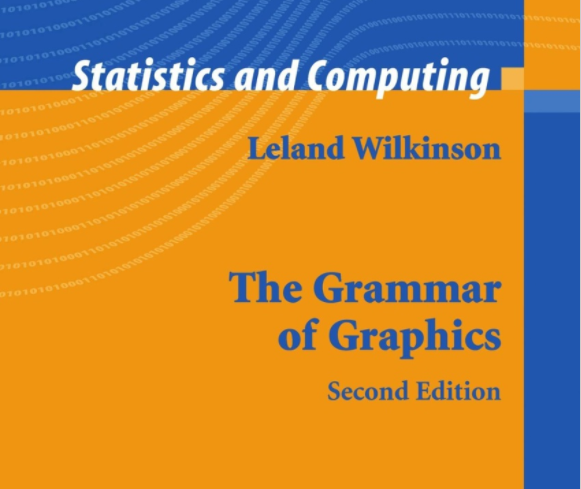
\includegraphics[width=0.70\linewidth]{PlotsLec2/GrammerOfGraphics}
\end{figure}
\end{frame}

%\setbeamercovered{transparent}
\begin{frame}{Grammar of English Language}
\begin{itemize}
\item Grammar provides the \textcolor{red}{key components} of a language, using which you can write
new sentences, essays, or best selling novels.
\item Take the example of the famous sentence (pangram):
\begin{equation*}
\text{\textcolor{red}{The quick brown fox jumps over the lazy dog.}}
\end{equation*}
\item Every word has a \textcolor{blue}{clear grammatical definition}:
\begin{figure}
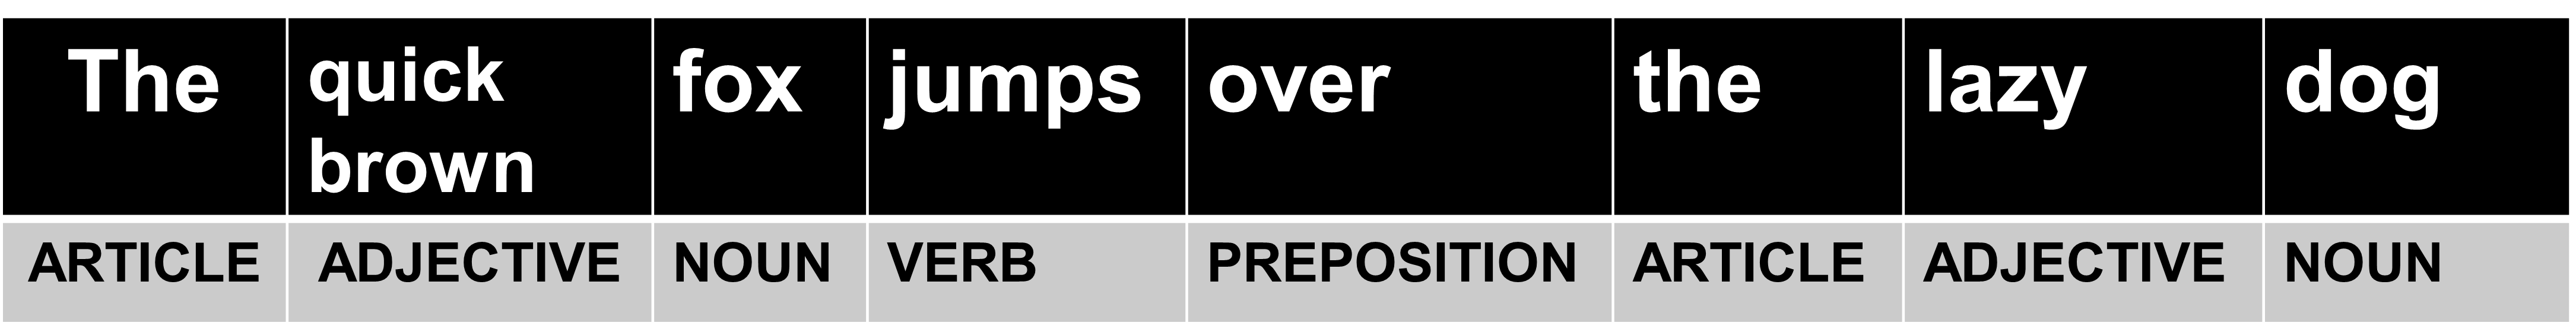
\includegraphics[width=0.99\linewidth]{PlotsLec2/QuickBrownFox}
\end{figure}
\item The sentence \textcolor{blue}{conveys a specific message}, and \textcolor{blue}{to change the message}, we need to \textcolor{blue}{change} its \textcolor{blue}{grammatical components}.
\end{itemize}
\end{frame}

\begin{frame}\frametitle{Grammar of Graphics}
The same framework holds true for creating visualisations in ggplot2 --- the grammer of graphics provides all the \textcolor{red}{individual components} (like noun, verb, and adjective) and the \textcolor{red}{rules to assemble} them for producing meaningful visualisations.
\begin{figure}
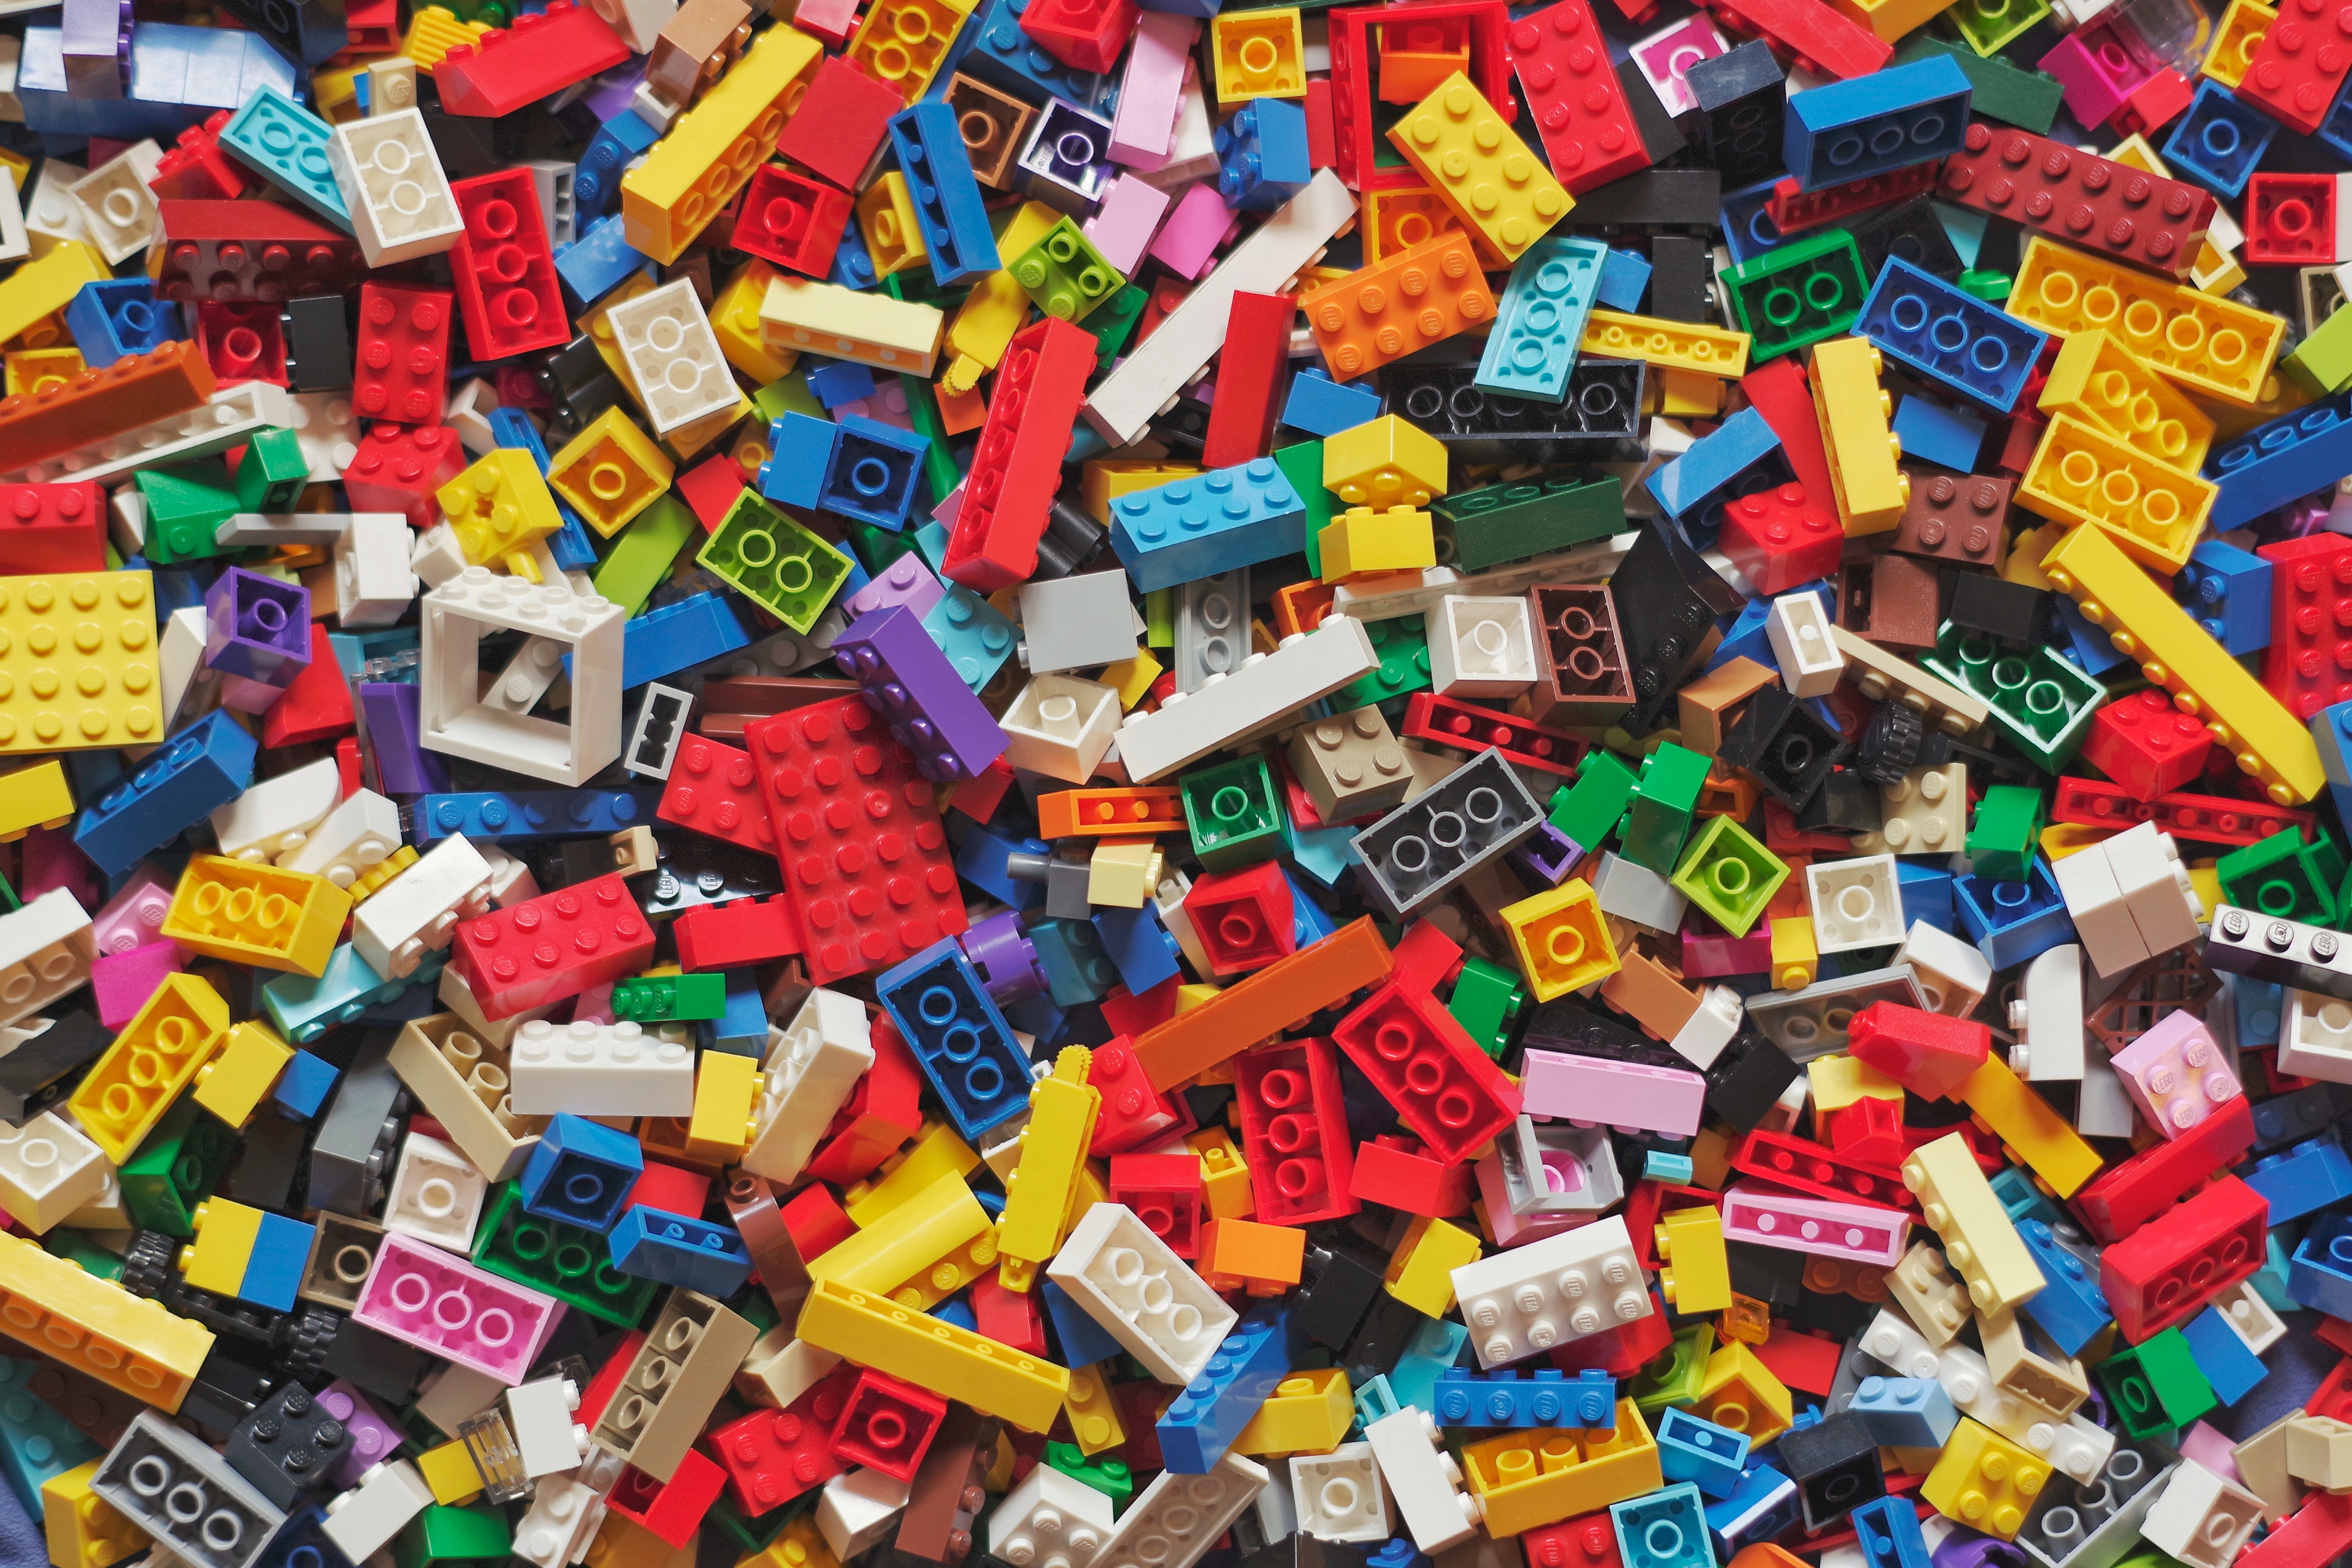
\includegraphics[width=0.75\linewidth]{PlotsLec2/Lego}
\end{figure}
\end{frame}


\begin{frame}[t]\frametitle{Ggplot2 is part of Tidyverse}
\small
The second reason is that Ggplot2 \textcolor{red}{works well with other R-packages} of Tidyverse --- this \textcolor{red}{saves time} in writing R-code for visualisation.
\begin{figure}
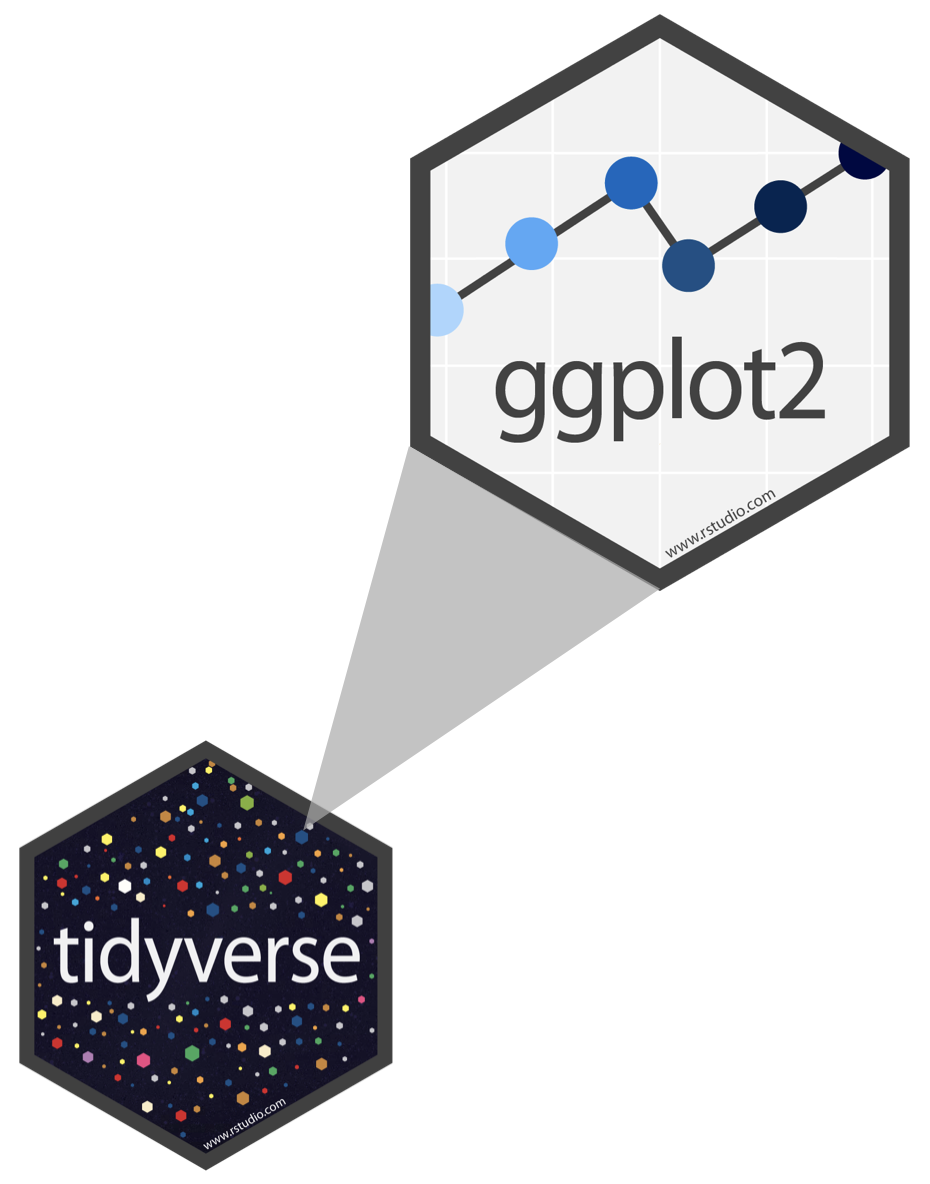
\includegraphics[width=0.50\linewidth]{PlotsLec2/ggplot2partoftidyverse}
\end{figure}
\end{frame}

\begin{frame}\frametitle{Several great resources available}
The third and last reason is that, great resources are available for ggplot2 --- ask questions on stackoverflow:
\textcolor{blue}{https://stackoverflow.com/questions/tagged/ggplot2}
\begin{figure}
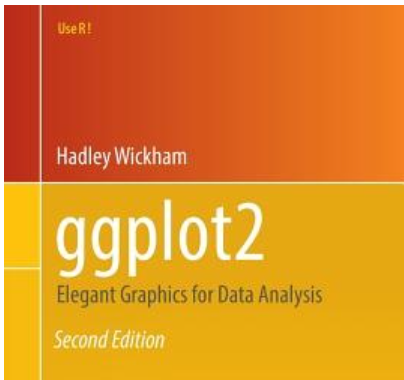
\includegraphics[width=0.60\linewidth]{PlotsLec2/ggplot2book}
\end{figure}
\end{frame}

\section{Key three elements of any Ggplot2 figure}
\begin{frame}\frametitle{Three essential components/layers}
The three essential components of any ggplot2 visualisation are: (i) \texttt{data}, (ii) \texttt{aes} (aesthetic mappings), and (iii) \texttt{geom}$\_\star$ (geometry).
\begin{figure}
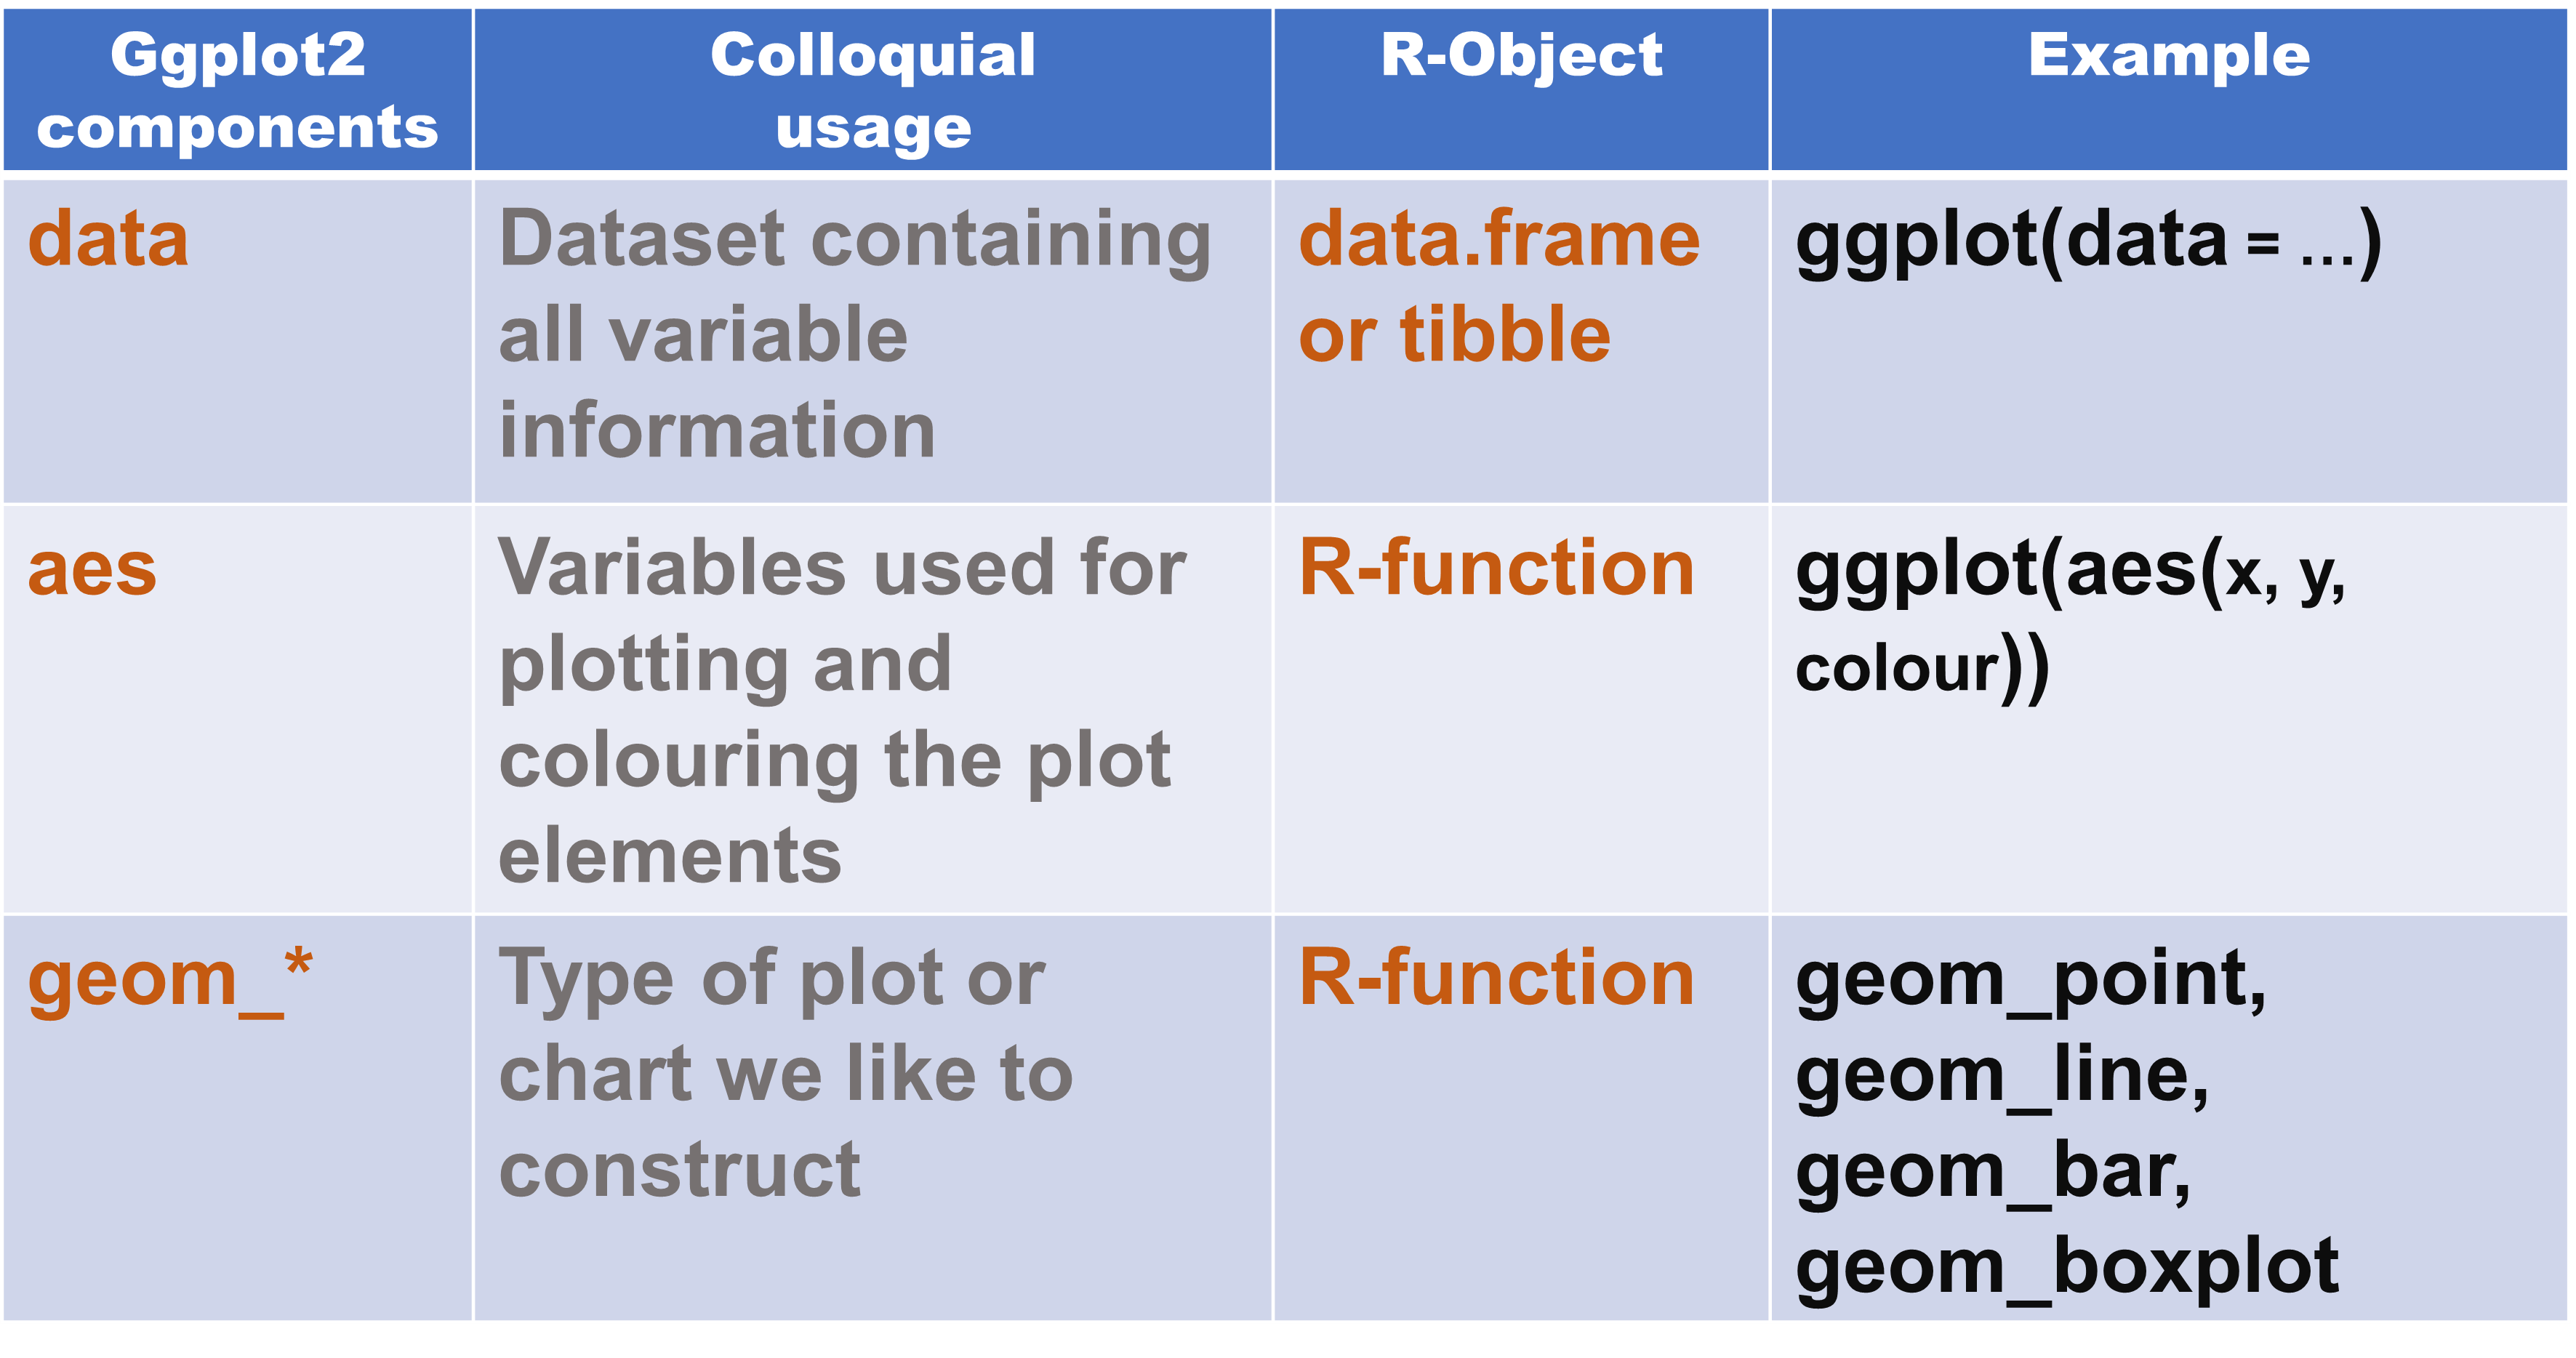
\includegraphics[width=0.99\linewidth]{PlotsLec2/MainComponents}
\end{figure}
\end{frame}

\begin{frame}\frametitle{Combining three essential layers}
We start with \textcolor{red}{\texttt{data}} layer, and add the \textcolor{red}{\texttt{aes}} layer on top of that, and finally, we add the \textcolor{red}{\texttt{geom}} layer on top. 
\begin{figure}
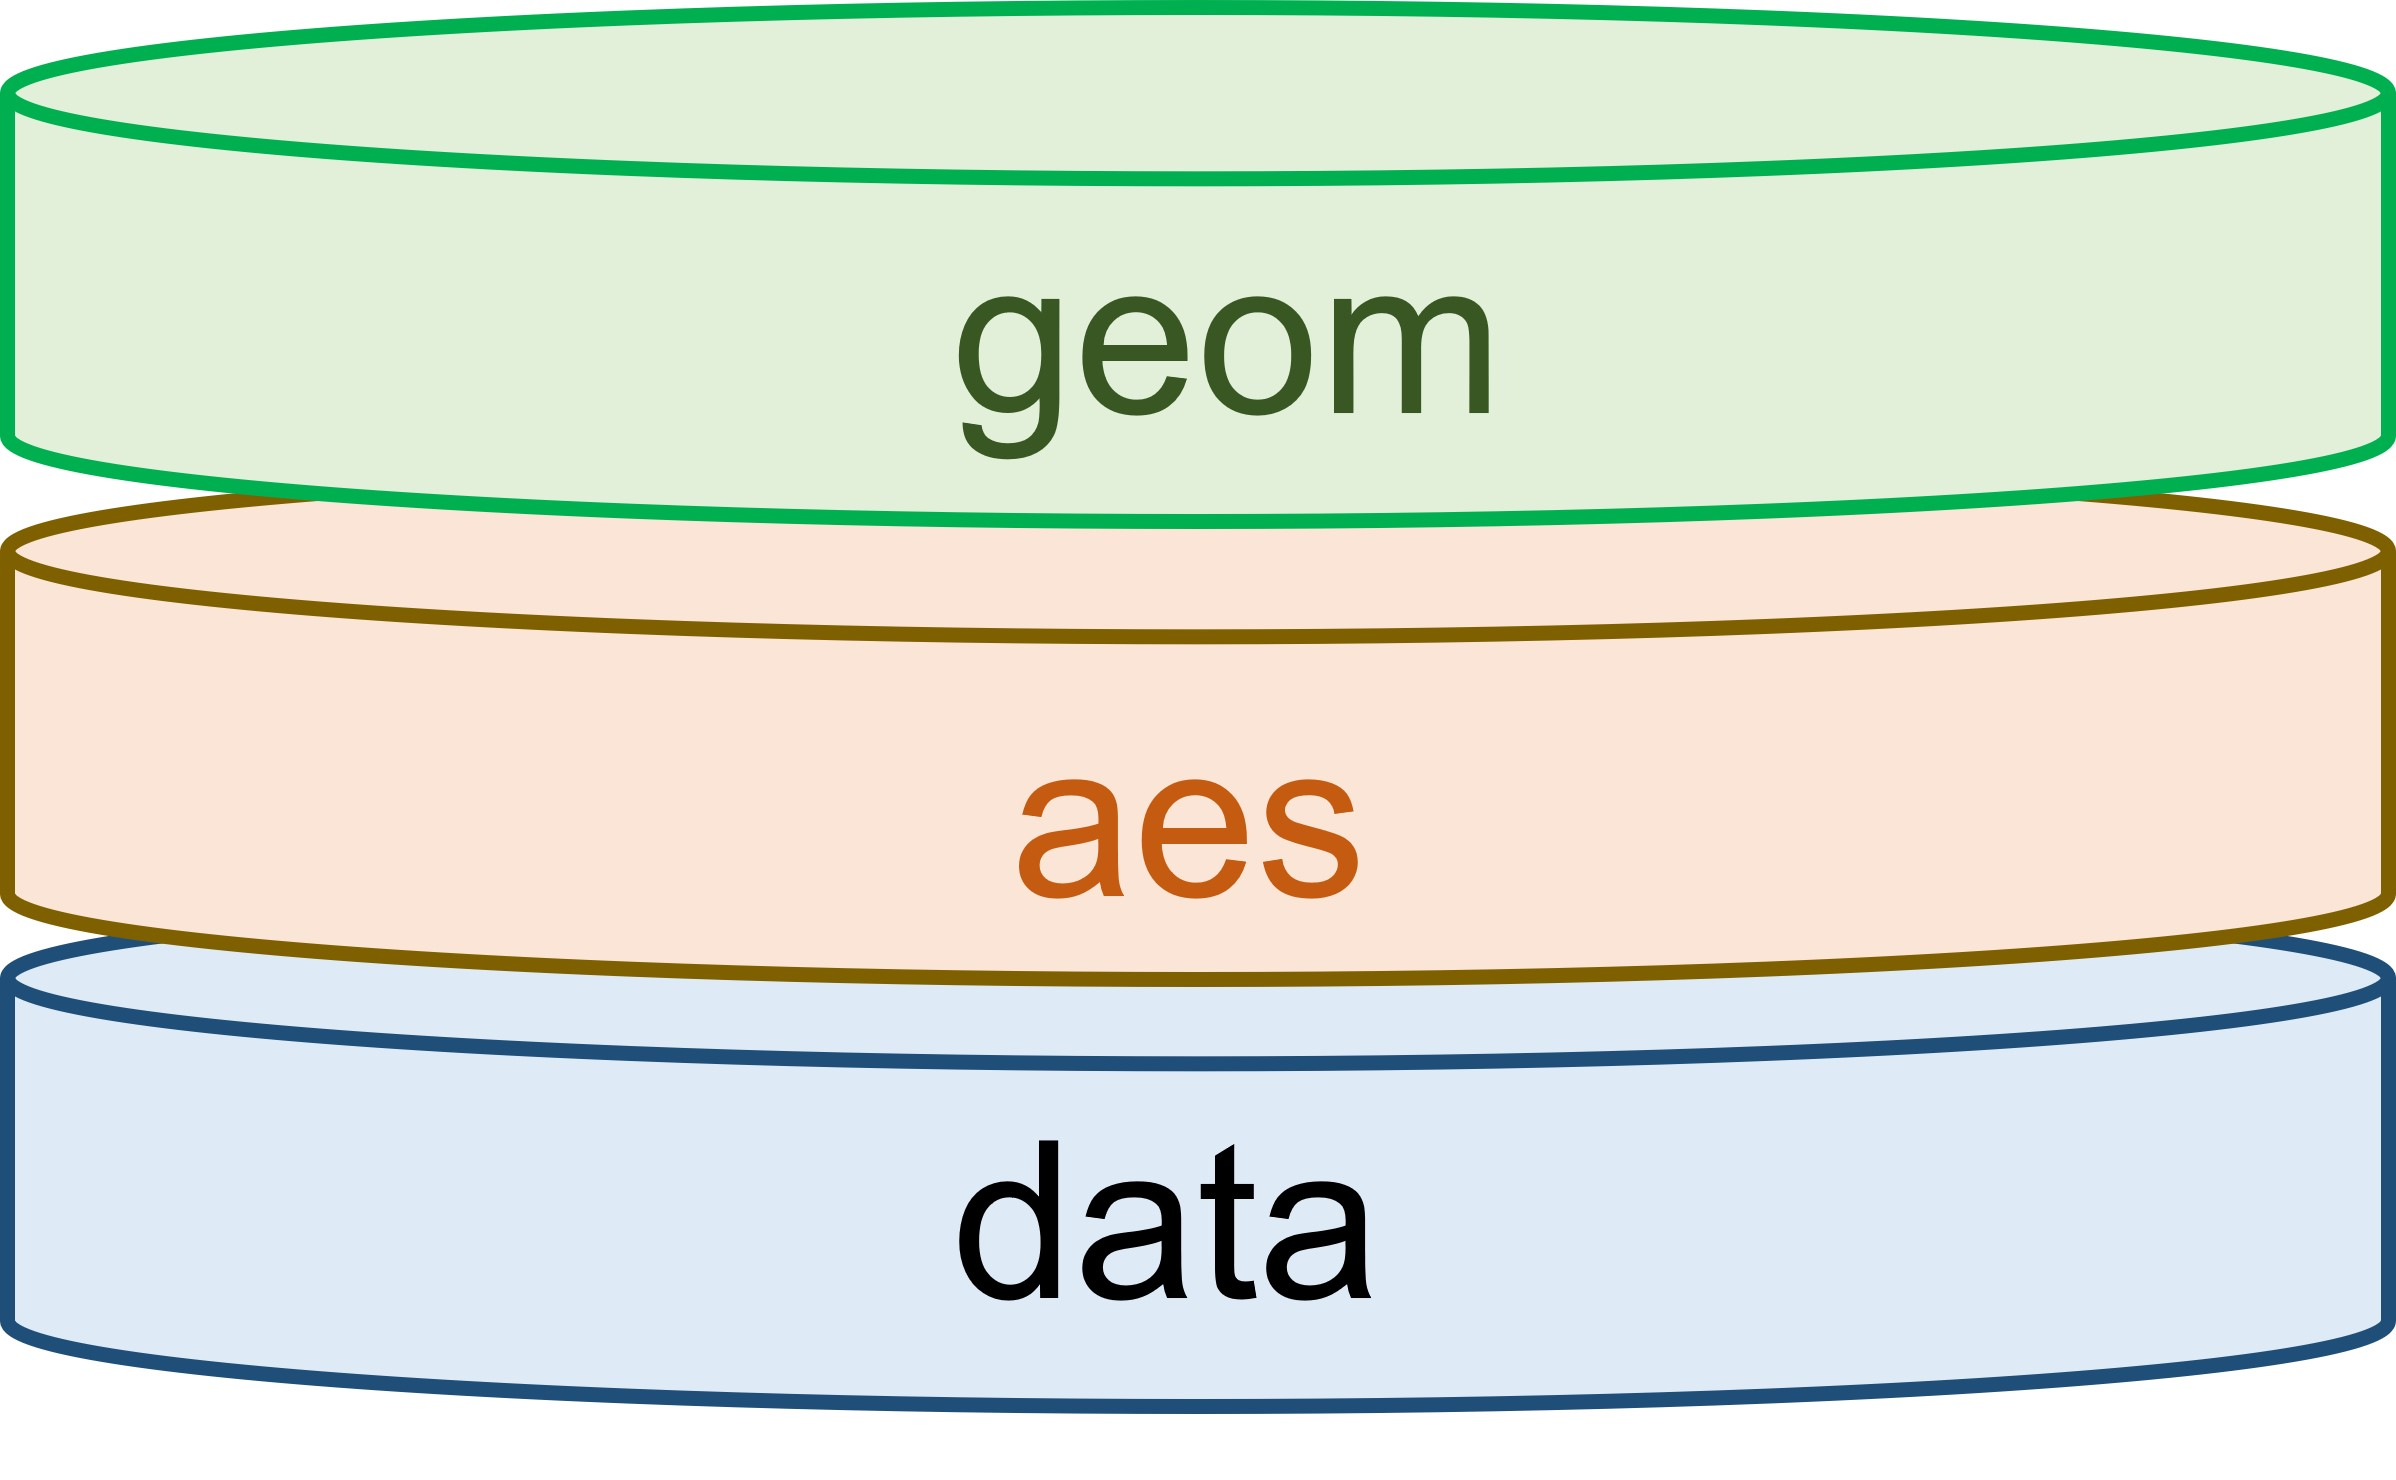
\includegraphics[width=0.99\linewidth]{PlotsLec2/GgplotLayers}
\end{figure}
\end{frame}


\section{Key element-1: Data}
\begin{frame}{Example: \textcolor{red}{Iris} dataset}
We can use \textcolor{red}{the three main components} of ggplot2 to create a very quick exploratory plot using the iris dataset.
\begin{figure}
\includegraphics[width=0.99\linewidth]{PlotsLec2/IrisDataset}
\end{figure}
We like to \textcolor{red}{investigate the relationship between Sepal.Length and Sepal.Width}.
\end{frame}

\begin{frame}\frametitle{Iris data: Sepal.Length versus Sepal.Width}
\begin{figure}
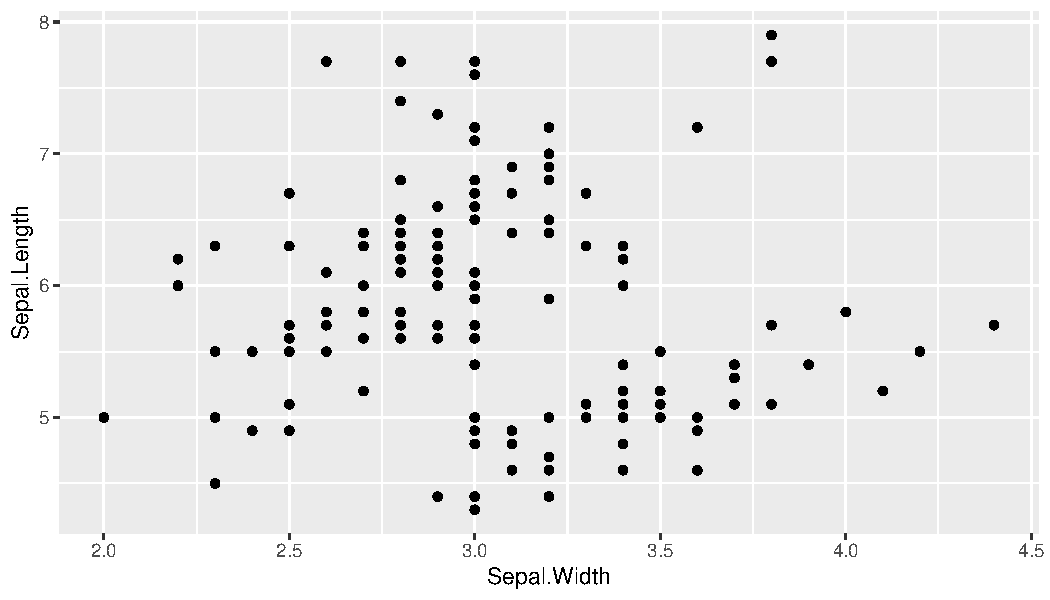
\includegraphics[width=0.99\linewidth]{PlotsLec2/Scatter1}
\caption{{\small Barebone scatter plot of Sepal.Length versus Sepal.Width \textcolor{red}{using three main components} of ggplot2.}}
\end{figure}
\end{frame}

\begin{frame}\frametitle{Can you guess the code?}
\Large
\begin{itemize}
\item What is the \textcolor{red}{data} component?
\vspace{0.3in}
\item What are the \textcolor{red}{aesthetic} mappings?
\vspace{0.3in}
\item What is the \textcolor{red}{geometry} component?
\end{itemize}
\end{frame}

\begin{frame}[fragile]\frametitle{Ggplot2 code of scatter plot}
%\lstset{basicstyle=\tiny\ttfamily}
\begin{lstlisting}
# Sepal.Length versus Sepal.Width
ggplot(data = iris,
       mapping=aes(x = Sepal.Width, 
                   y = Sepal.Length)) +
       geom_point()
\end{lstlisting}

\begin{lstlisting}
# Shorter version of the same code
iris %>%
ggplot(aes(Sepal.Width, Sepal.Length)) +
geom_point()
\end{lstlisting}
\end{frame}

\begin{frame}\frametitle{Let's see another example: \textcolor{red}{mtcars}}
\begin{figure}
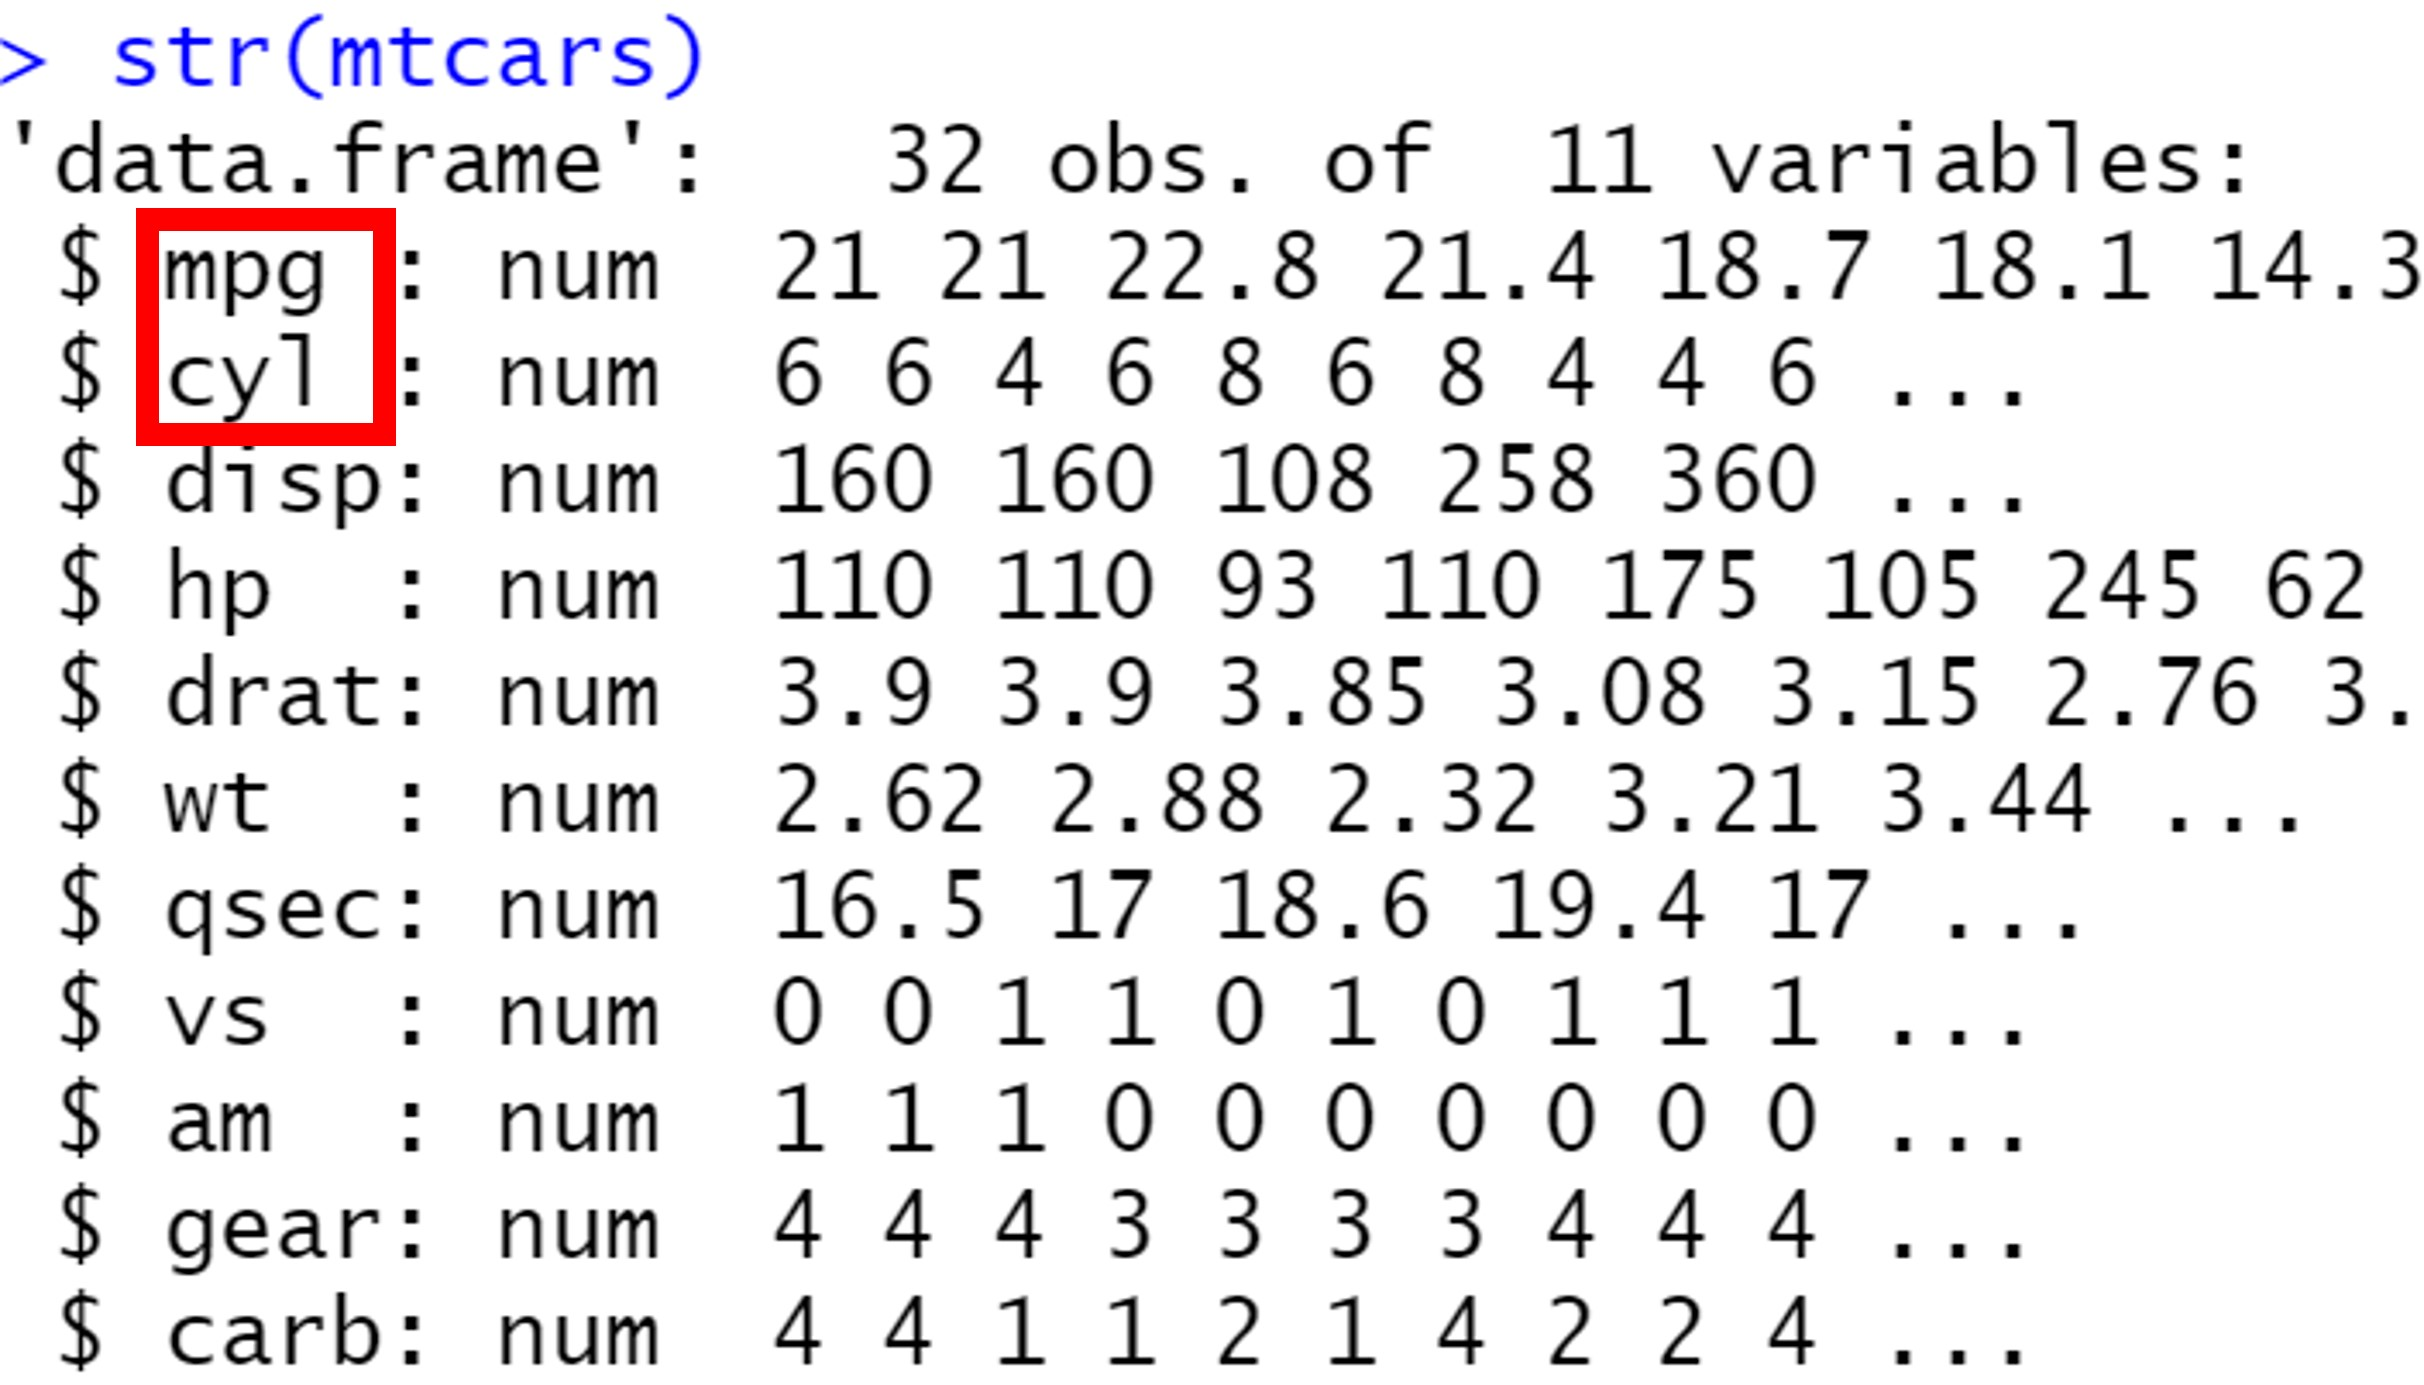
\includegraphics[width=0.99\linewidth]{PlotsLec2/mtcars}
\caption{{\small Aim is to investigate the relationship between \textcolor{red}{mpg} (miles per gallon) and \textcolor{red}{cyl} (number of cylinders).}}
\end{figure}
\end{frame}


\section{Key element-2: Aesthetics}
\begin{frame}[fragile]\frametitle{RCode --- scatter plot of \textcolor{red}{mpg} against \textcolor{red}{cyl}}
we start with the \textcolor{red}{\texttt{mtcars}} data layer. We map \textcolor{red}{cyl} to $x$-axis aesthetics and \textcolor{red}{mpg} to $y$-axis aesthetics. For obtaining a scatter plot, we add the \textcolor{red}{\texttt{geom}$\_$\texttt{point()}} layer on top.
\lstset{basicstyle=\Large\ttfamily}
\begin{lstlisting}
# Scatter plot: mpg versus cyl
mtcars %>%
ggplot(aes(x= cyl, y = mpg)) +
geom_point()
\end{lstlisting}
\end{frame}

\begin{frame}\frametitle{Scatter plot: \textcolor{red}{mpg} versus \textcolor{red}{cyl}}
\textcolor{blue}{Can you spot any problem with this plot}?
\begin{figure}
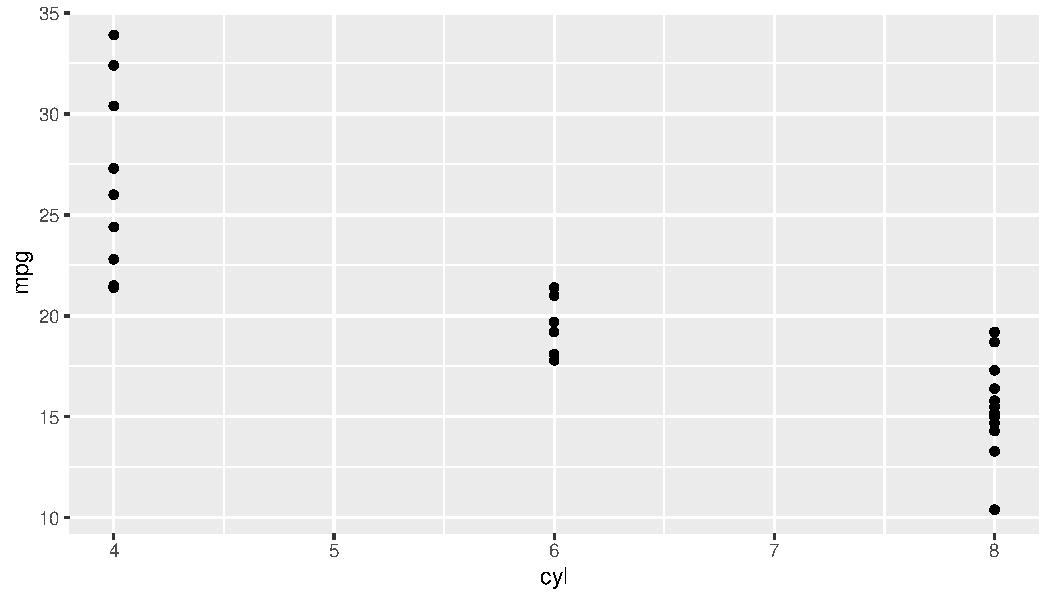
\includegraphics[width=0.99\linewidth]{PlotsLec2/mpg_vs_cyl}
\end{figure}
\end{frame}



\begin{frame}[fragile]\frametitle{\textcolor{red}{cyl} should be a categorical variable}
\lstset{basicstyle=\small\ttfamily}
\begin{lstlisting}
mtcars %>%
ggplot(aes(as.character(cyl), mpg)) +
geom_point()
\end{lstlisting}
\begin{figure}
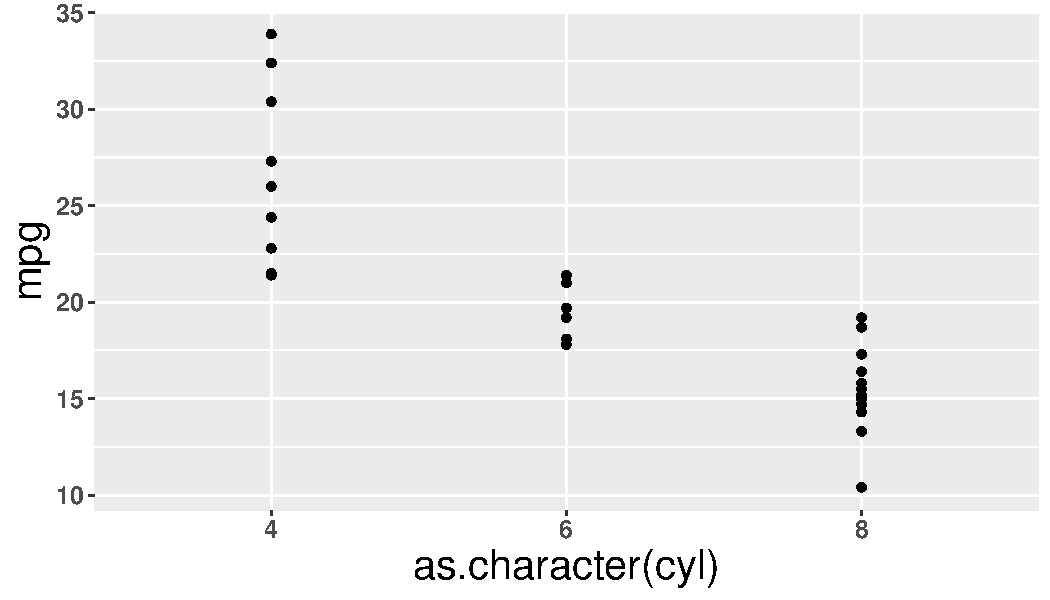
\includegraphics[width=0.90\linewidth]{PlotsLec2/mpg_vs_cyl2}
\caption{{\small\textcolor{red}{cyl} levels are ordered alphabetically.}}
\end{figure}
\end{frame}

\begin{frame}[fragile]\frametitle{Use \textcolor{red}{\texttt{factor()}} to convert \textcolor{red}{cyl}}
Use \textcolor{red}{\texttt{factor()}} rather than \textcolor{red}{\texttt{as.character()}} to turn \textcolor{red}{\texttt{cyl}} into a categorical variable

\begin{lstlisting}
mtcars %>%
ggplot(aes(factor(cyl), mpg)) +
geom_point()
\end{lstlisting}

\begin{figure}
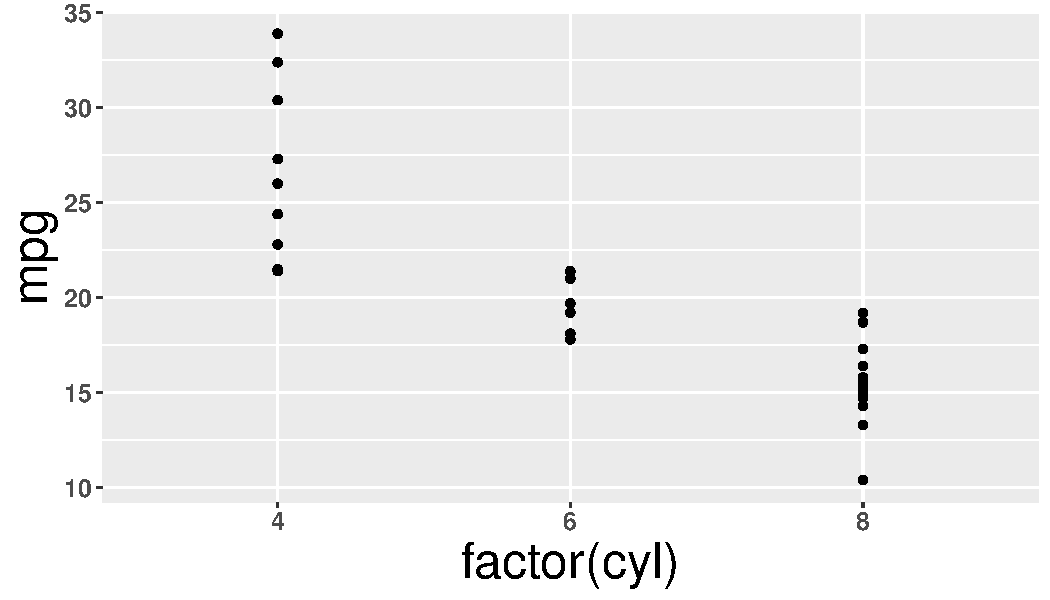
\includegraphics[width=0.75\linewidth]{PlotsLec2/mpg_vs_cyl3}
\end{figure}
\end{frame}

\begin{frame}\frametitle{Advantage of using \texttt{factor}?}
\Large
What is the advantage of using \textcolor{red}{\texttt{factor()}} instead of \textcolor{red}{\texttt{as.character()}}?
\end{frame}

\begin{frame}[fragile]\frametitle{Ordering levels of categorical variables}
You can \textcolor{red}{change the default ordering of the levels} of a categorical variable using \textcolor{red}{\texttt{factor()}}. 
\begin{figure}
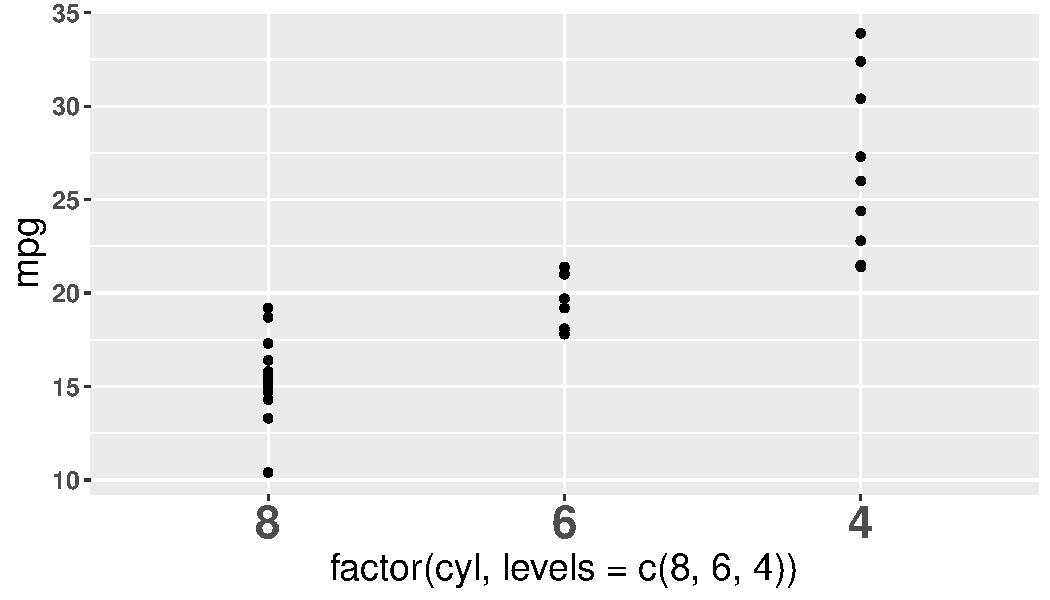
\includegraphics[width=0.99\linewidth]{PlotsLec2/mpg_vs_cyl4}
\end{figure}
\end{frame}

\begin{frame}\frametitle{More \textcolor{blue}{\texttt{aes}} mapping: \textcolor{red}{\texttt{color}}, \textcolor{red}{\texttt{size}}, and \textcolor{red}{\texttt{fill}}}
\begin{itemize}
\item We learnt about the aesthetic mappings onto the \textcolor{red}{\texttt{x}} and \textcolor{red}{\texttt{y}} axes.
\item The \textcolor{blue}{next three most useful} aesthetic mappings are \textcolor{red}{\texttt{color}}, \textcolor{red}{\texttt{size}}, and \textcolor{red}{\texttt{fill}}.
\end{itemize}
\begin{figure}
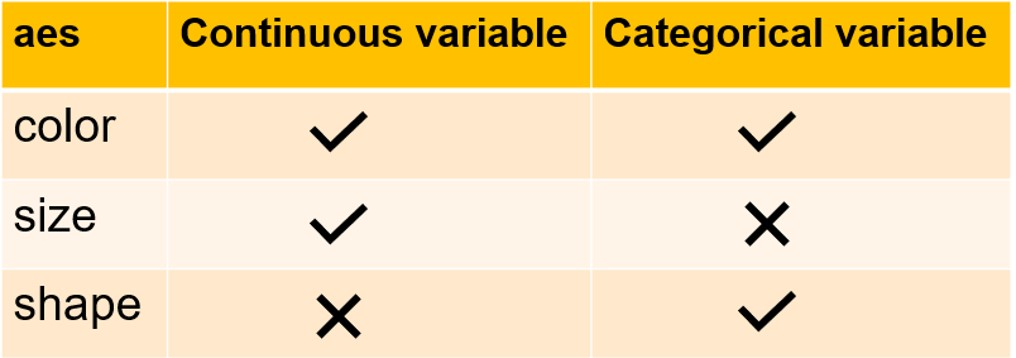
\includegraphics[width=0.99\linewidth]{PlotsLec2/AesChecks}
\end{figure}
\end{frame}

\begin{frame}\frametitle{Map categorical \textcolor{blue}{\texttt{cyl}} onto  \textcolor{red}{\texttt{color}} aesthetic}
\Large
\textcolor{red}{Aim}: Use \textcolor{blue}{\texttt{mtcars}} \textcolor{red}{\texttt{data layer}} to investigate how \textcolor{blue}{\texttt{disp}} (engine displacement measured in cubic inches) influences \textcolor{blue}{\texttt{mpg}} (miles per gallon) for different \textcolor{blue}{\texttt{cyl}} (number of cylinders) values.
\end{frame}


\begin{frame}[fragile]\frametitle{RCode: map categorical \textcolor{blue}{\texttt{cyl}} onto  \textcolor{red}{\texttt{color}}}
{\Large Note the \textcolor{red}{\texttt{color}} aesthetic inside the \textcolor{blue}{\texttt{aes}} function.}

\lstset{basicstyle=\Large\ttfamily}
\begin{lstlisting}
# Scatter plot: mpg versus disp
mtcars %>%
ggplot(aes(x= disp, 
           y = mpg,
        color = factor(cyl))) +
geom_point()
\end{lstlisting}
\end{frame}

\begin{frame}\frametitle{Mapping categorical \textcolor{blue}{\texttt{cyl}} onto  \textcolor{red}{\texttt{color}}}
\textcolor{red}{Legend title} reflects the mapping of \textcolor{blue}{\texttt{cyl}} onto  \textcolor{red}{\texttt{color}}. 
\begin{figure}
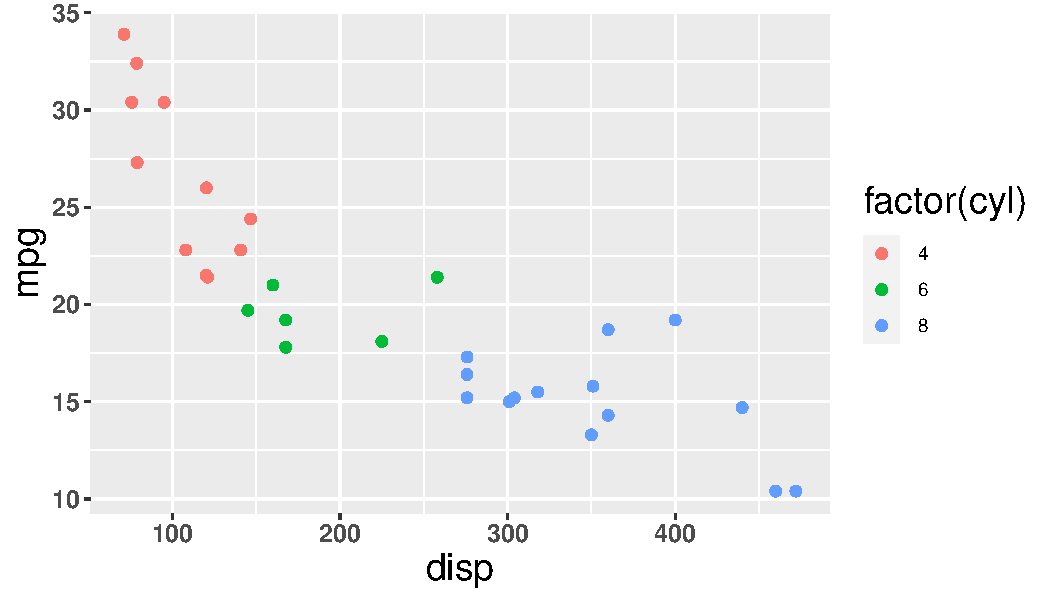
\includegraphics[width=0.99\linewidth]{PlotsLec2/cyl_to_color}
\caption{{\small Cars with larger \textcolor{blue}{\texttt{cyl}} values are less fuel-efficient (low \textcolor{blue}{\texttt{mpg}}) but exhibit higher engine displacement (\textcolor{blue}{\texttt{disp}}).}}
\end{figure}
\end{frame}

\begin{frame}[fragile]\frametitle{Mapping continuous \textcolor{blue}{\texttt{disp}} onto  \textcolor{red}{\texttt{color}}}
\textcolor{red}{Gradient color scheme} reflects the mapping of the continuous \textcolor{blue}{\texttt{disp}} onto \textcolor{red}{\texttt{color}}. 
\begin{figure}
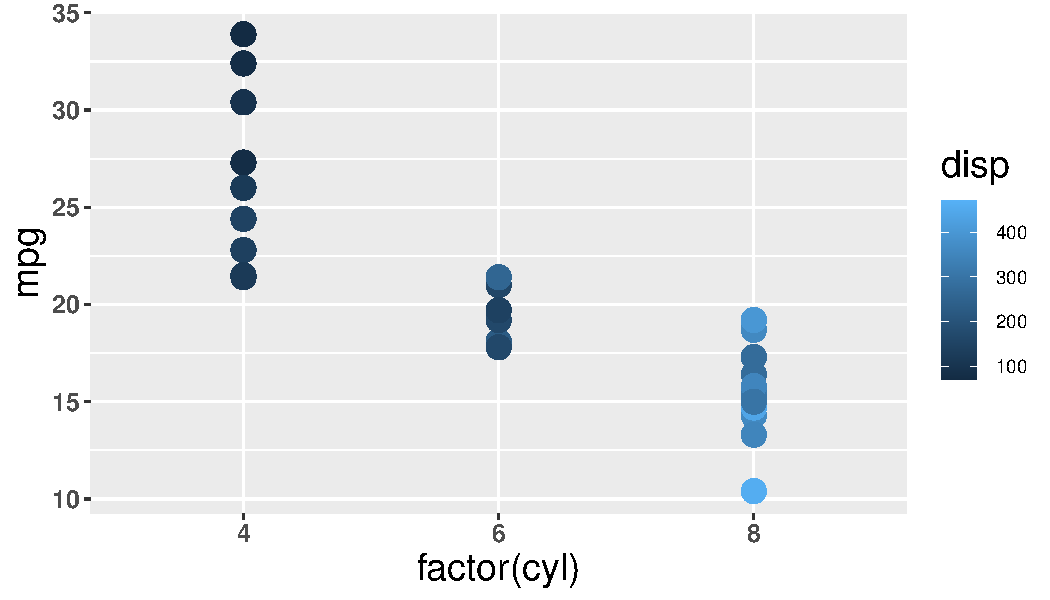
\includegraphics[width=0.99\linewidth]{PlotsLec2/disp_to_color}
\caption{{\small The value of \textcolor{blue}{\texttt{disp}} gradually increases as the shade of blue gets from darker to lighter.}}
\end{figure}
\end{frame}

\begin{frame}\frametitle{Example data: \texttt{\textcolor{red}{mpg}} from \texttt{\textcolor{red}{ggplot2}}}
\begin{figure}
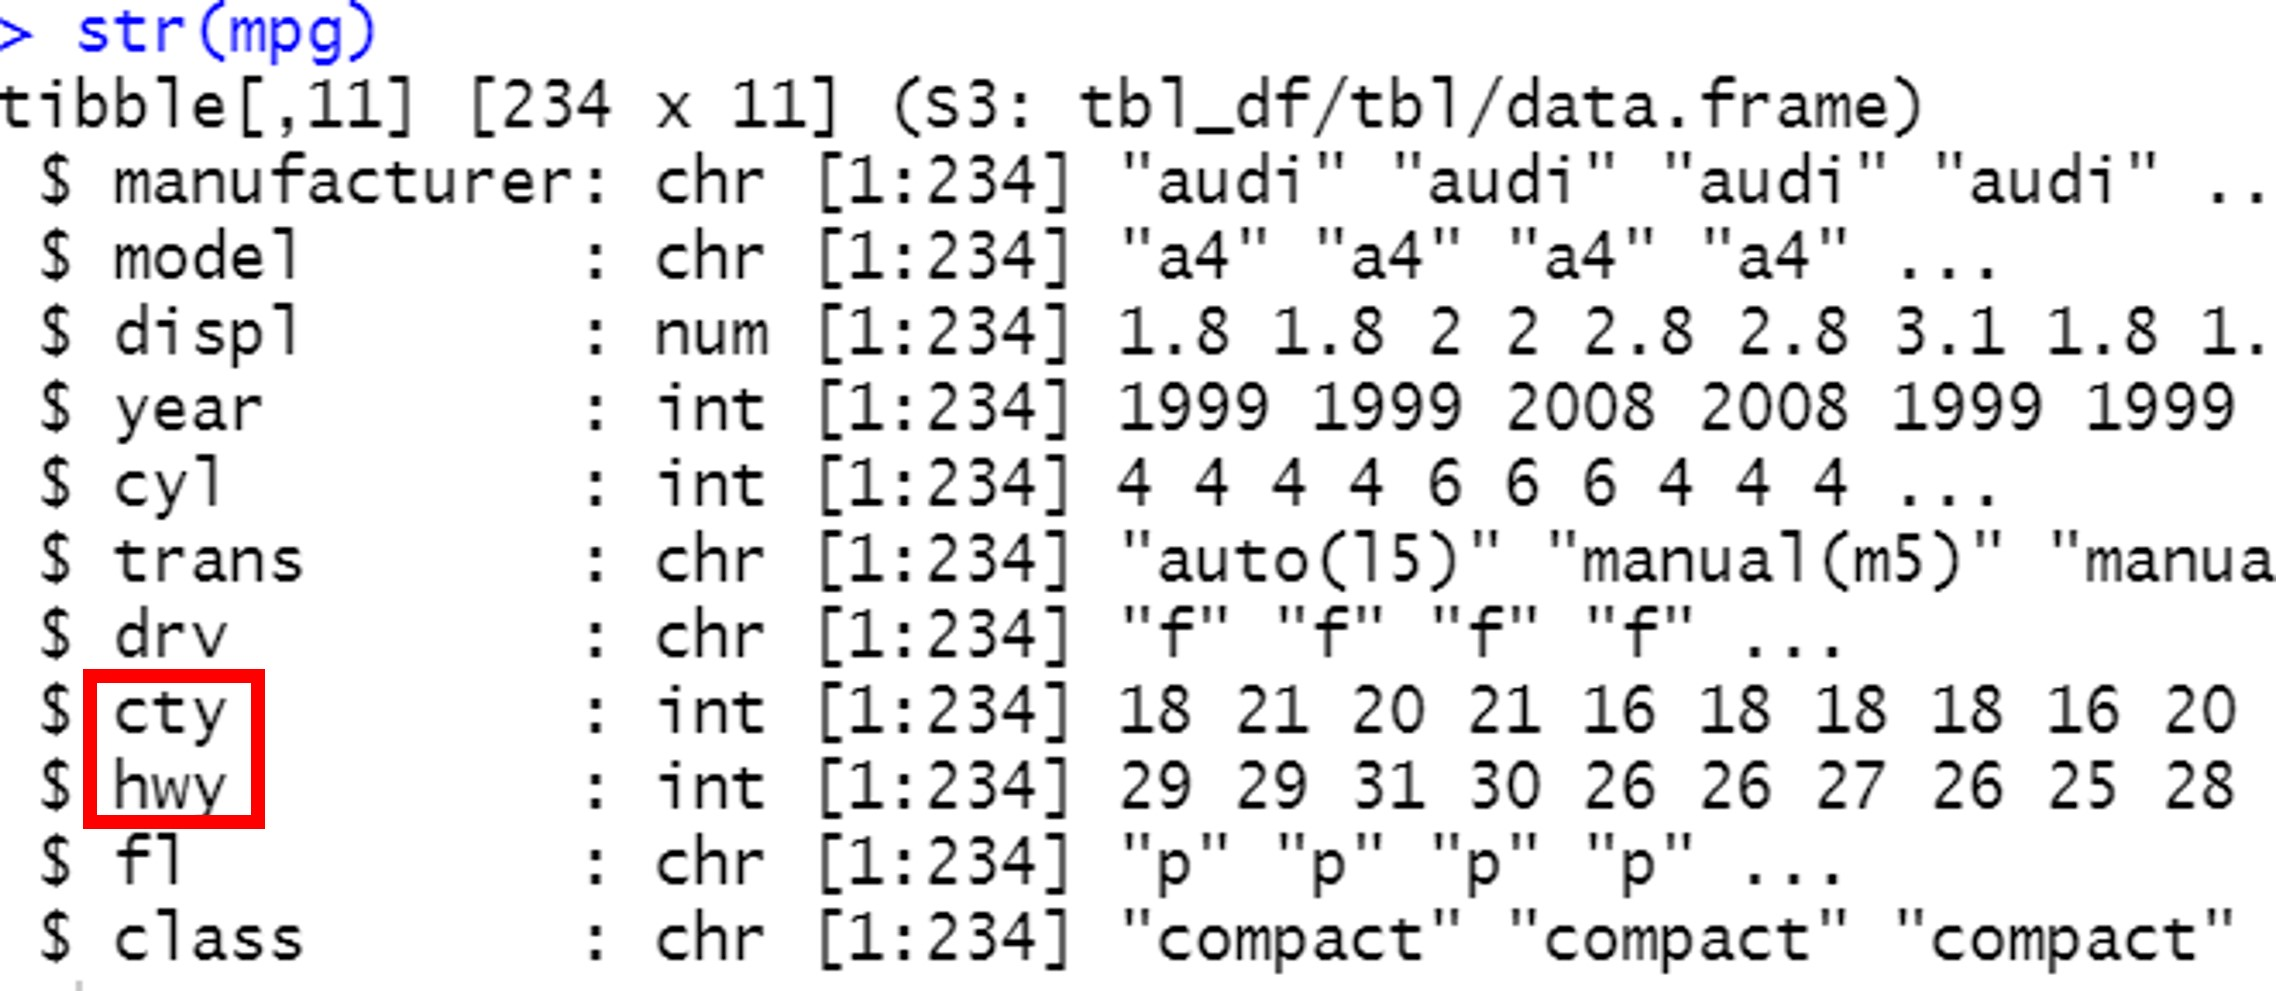
\includegraphics[width=0.99\linewidth]{PlotsLec2/mpg}
\caption{{\small Aim is to investigate \textit{\textcolor{blue}{highway miles per gallon}} (\texttt{\textcolor{red}{hwy}}) as a function of \textit{\textcolor{blue}{city miles per gallon}} (\texttt{\textcolor{red}{cty}}).}}
\end{figure}
\end{frame}

\begin{frame}[fragile]\frametitle{RCode: mapping continuous \texttt{\textcolor{blue}{displ}} to \texttt{\textcolor{red}{size}}}
{\Large Note the \textcolor{red}{\texttt{size}} aesthetic inside the \textcolor{blue}{\texttt{aes()}} function, and also the new \textcolor{red}{\texttt{geom}} layer.}

\lstset{basicstyle=\Large\ttfamily}
\begin{lstlisting}
# Scatter plot: hwy versus cty
mpg %>%
ggplot(aes(x = cty, 
           y = hwy,
        size = displ)) +
geom_jitter()
\end{lstlisting}
\end{frame}

\begin{frame}\frametitle{Scatter plot: \texttt{\textcolor{blue}{displ}} mapped to \texttt{\textcolor{red}{size}}}
\begin{figure}
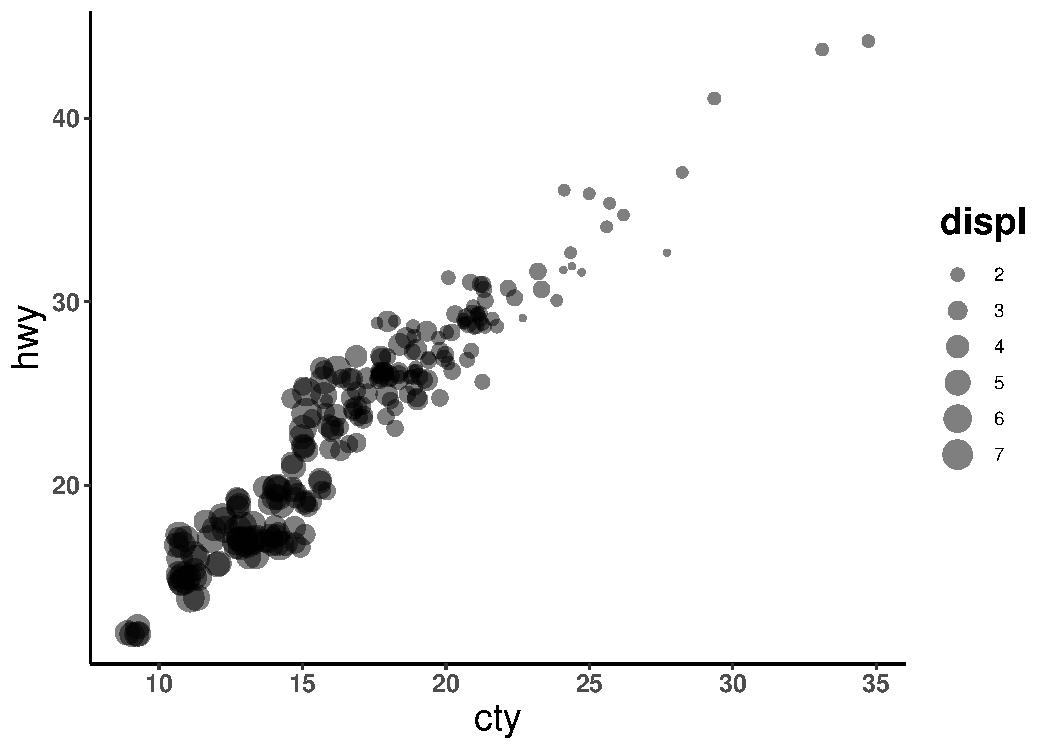
\includegraphics[width=0.99\linewidth]{PlotsLec2/displ_to_size}
\end{figure}
\end{frame}



\begin{frame}\frametitle{Avoid mapping \texttt{\textcolor{blue}{factors}} onto \texttt{\textcolor{red}{size}}}
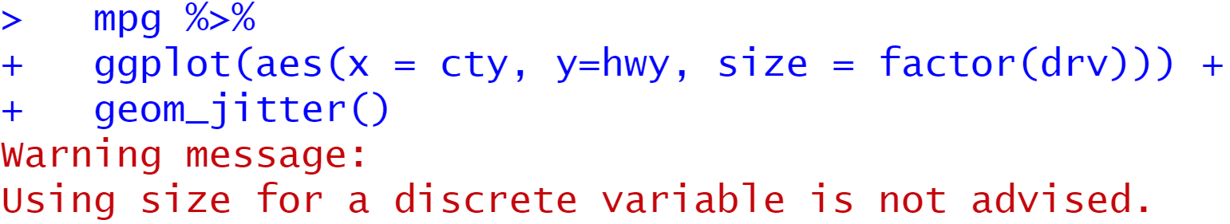
\includegraphics[width=0.99\linewidth]{PlotsLec2/Warning1}
\end{frame}

\begin{frame}\frametitle{Example: map \texttt{\textcolor{blue}{factors}} onto \texttt{\textcolor{red}{shape}}}
\begin{figure}
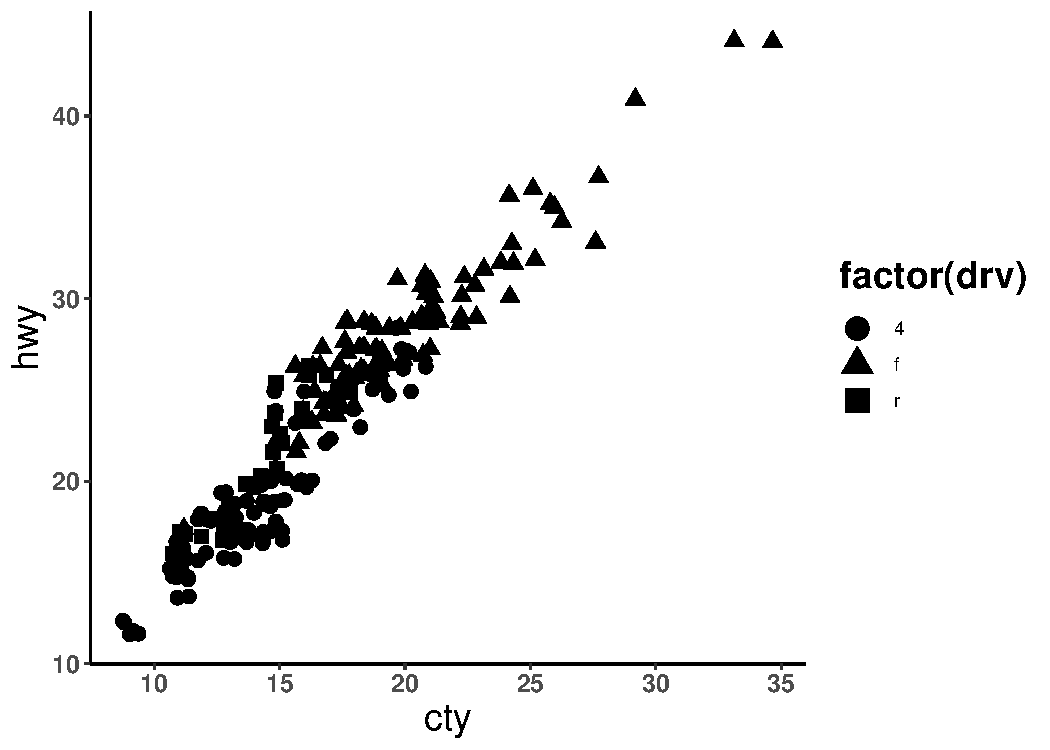
\includegraphics[width=0.90\linewidth]{PlotsLec2/drv_to_shape}
\caption{{\small Hard to distinguish between four wheel (\textcolor{red}{\texttt{4}}) and rear wheel (\textcolor{red}{\texttt{r}}) drives.}}
\end{figure}
\end{frame}

\begin{frame}\frametitle{\textcolor{red}{Faceting} --- conditional plots}
The best way to investigate the relationship between \texttt{\textcolor{blue}{hwy}} and \texttt{\textcolor{blue}{cty}} for the three driving categories (\texttt{\textcolor{blue}{drv}}) is by using the \texttt{\textcolor{red}{facet}$\_$\textcolor{red}{wrap()}} function.
\begin{figure}
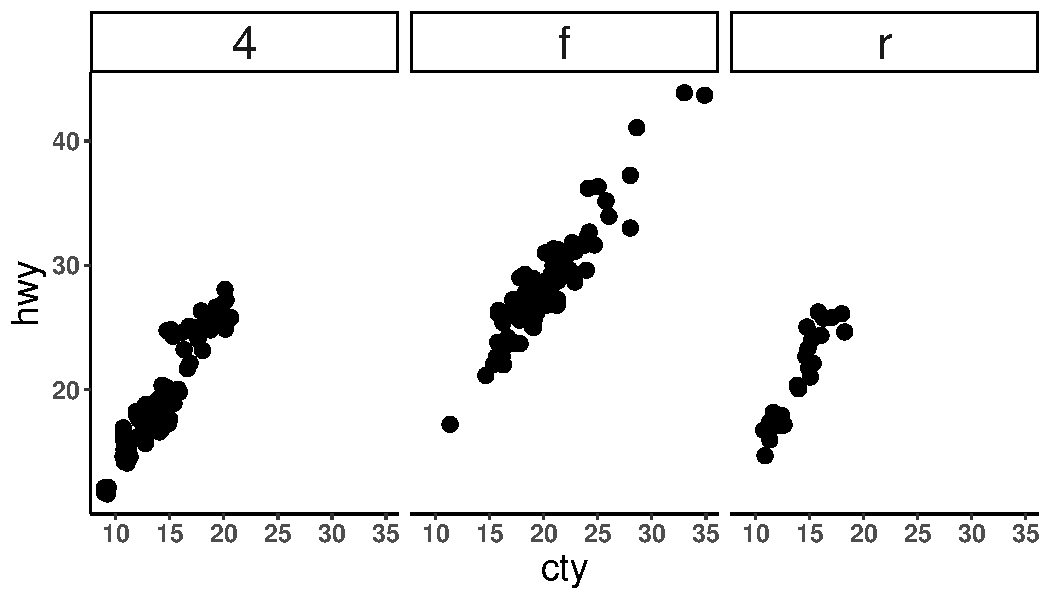
\includegraphics[width=0.99\linewidth]{PlotsLec2/facet1}
\end{figure}
\end{frame}

\begin{frame}[fragile]\frametitle{RCode: \texttt{\textcolor{red}{facet}$\_$\textcolor{red}{wrap()}} example}
\lstset{basicstyle=\Large\ttfamily}
\begin{lstlisting}
# Scatter plot: hwy versus cty
mpg %>%
ggplot(aes(x = cty, y = hwy)) +
geom_jitter() +
facet_wrap(~ factor(drv))
\end{lstlisting}
\end{frame}

\begin{frame}\frametitle{\texttt{\textcolor{red}{facet}$\_$\textcolor{red}{wrap()}} versus \texttt{\textcolor{red}{facet}$\_$\textcolor{red}{grid()}}}
\begin{figure}
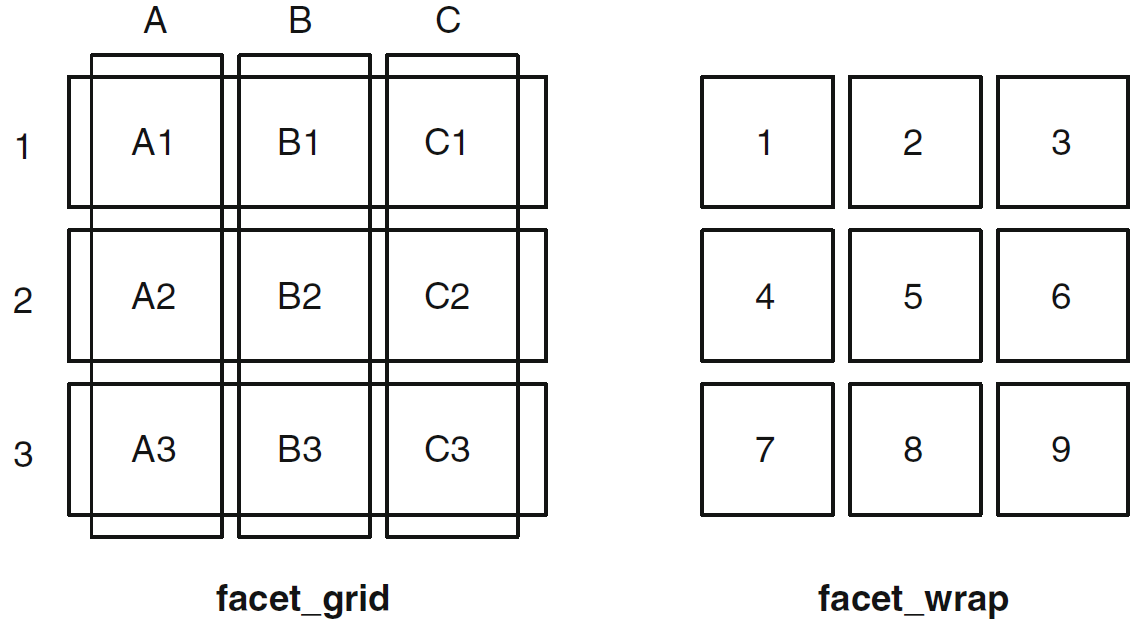
\includegraphics[width=0.99\linewidth]{PlotsLec2/FacettingInR}
\caption{{\small \texttt{\textcolor{red}{facet}$\_$\textcolor{red}{grid()}} is appropriate for including two factors into faceting --- from both \textcolor{blue}{row} and \textcolor{blue}{column} directions.}}
\end{figure}
\end{frame}

\begin{frame}\frametitle{Faceting using \texttt{\textcolor{red}{facet}$\_$\textcolor{red}{grid()}}}
\begin{figure}
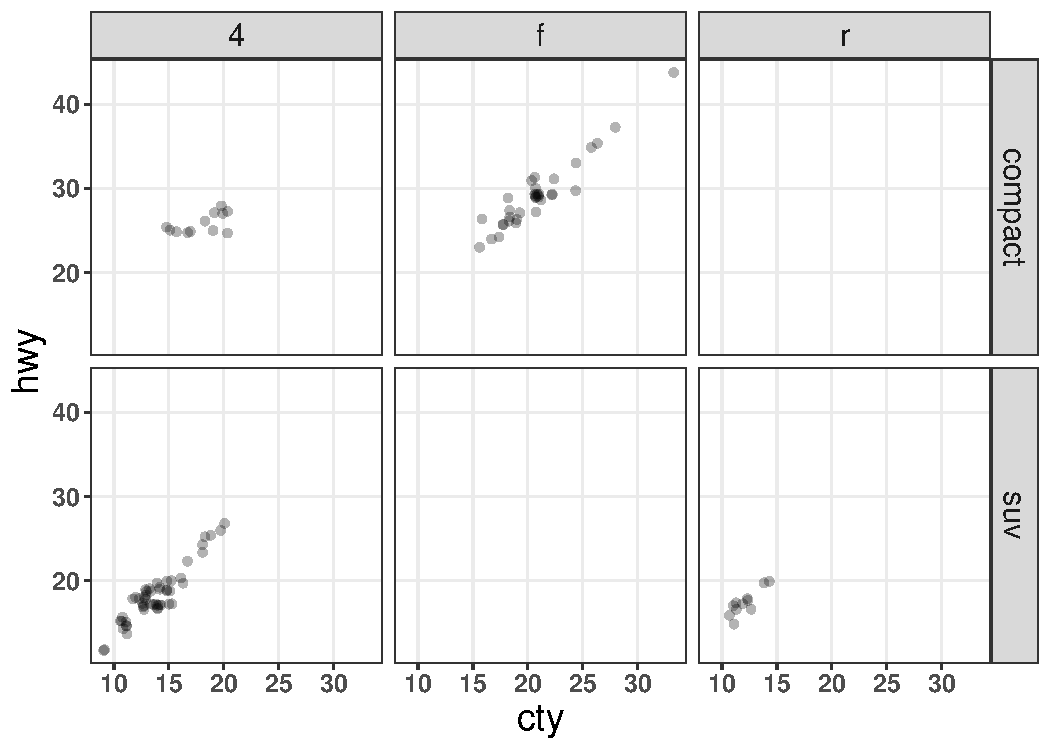
\includegraphics[width=0.99\linewidth]{PlotsLec2/facet_grid_example}
\caption{{\small \texttt{\textcolor{red}{hwy}} vs \texttt{\textcolor{red}{cty}} vs \texttt{\textcolor{red}{drv}} vs \texttt{\textcolor{red}{class}}.}}
\end{figure}
\end{frame}

\begin{frame}[fragile]\frametitle{RCode: \texttt{\textcolor{red}{facet}$\_$\textcolor{red}{grid()}} example}
\lstset{basicstyle=\Large\ttfamily}
\begin{lstlisting}
# Scatter plot: hwy versus cty
mpg %>%
ggplot(aes(x = cty, y = hwy)) +
geom_jitter() +
facet_grid(class ~ drv)
\end{lstlisting}
\end{frame}

\setbeamercovered{transparent}
\begin{frame}\frametitle{\textcolor{red}{\texttt{color}} versus \textcolor{red}{\texttt{fill}} aesthetics}
\begin{itemize}
\item Often there is a confusion between the \textcolor{red}{\texttt{color}} aesthetic and the \textcolor{red}{\texttt{fill}} aesthetic.
\vspace{0.3in}
\item<2-> \textcolor{red}{\texttt{color}} aesthetic typically changes the color of the outline of a plotting object.
\vspace{0.3in}
\item<3-> \textcolor{red}{\texttt{fill}} aesthetic changes the color of the body of a plotting object.
\end{itemize}
\end{frame}

\begin{frame}\frametitle{Example: \textcolor{red}{\texttt{color}} versus \textcolor{red}{\texttt{fill}} aesthetics}
\begin{figure}
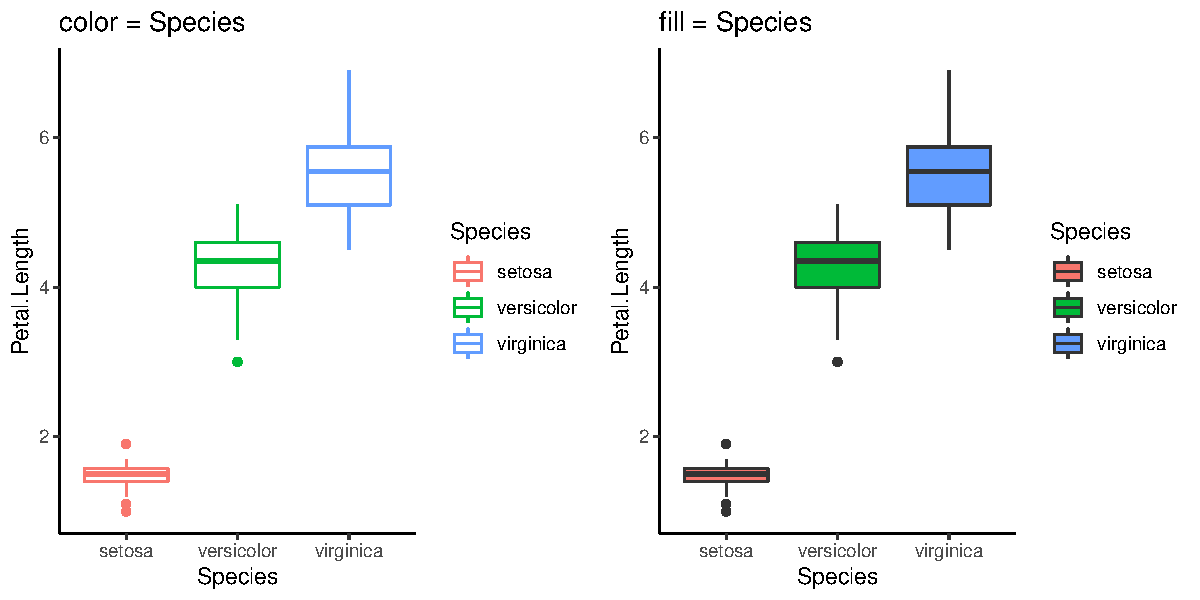
\includegraphics[width=0.99\linewidth]{PlotsLec2/bxplt_ex1}
\caption{\small{Boxplots of Petal.Length for three iris species using \textcolor{red}{\texttt{color = Species}} (\textit{left}) and \textcolor{red}{\texttt{fill = Species}} (\textit{right}).}}
\end{figure}
\end{frame}

\begin{frame}[fragile]\frametitle{RCode: \textcolor{red}{\texttt{color}} versus \textcolor{red}{\texttt{fill}} aesthetics}
\lstset{basicstyle=\Large\ttfamily}
\begin{lstlisting}
# Basic Boxplot: Petal.Length vs Species
base_plt <- ggplot(iris, aes(x = Species, y = Petal.Length))

# color = Species
base_plt + geom_boxplot(aes(color = Species))

# fill = Species
base_plt + geom_boxplot(aes(fill = Species))
\end{lstlisting}
\end{frame}

\begin{frame}\frametitle{Three key points from the last slide}
\Large
\begin{itemize}
\item Any ggplot \textcolor{red}{can be saved} as an R object/variable.
\vspace{0.3in}
\item ggplot objects \textcolor{red}{can be extended} using the \textcolor{blue}{\texttt{+}} operator.
\vspace{0.3in}
\item We \textcolor{red}{can call} \textcolor{blue}{\texttt{aes()}} \textcolor{red}{inside the geom layer} as well.
\end{itemize}
\end{frame}

\begin{frame}\frametitle{Example: \textcolor{red}{\texttt{color}} versus \textcolor{red}{\texttt{fill}} aesthetics}
\begin{figure}
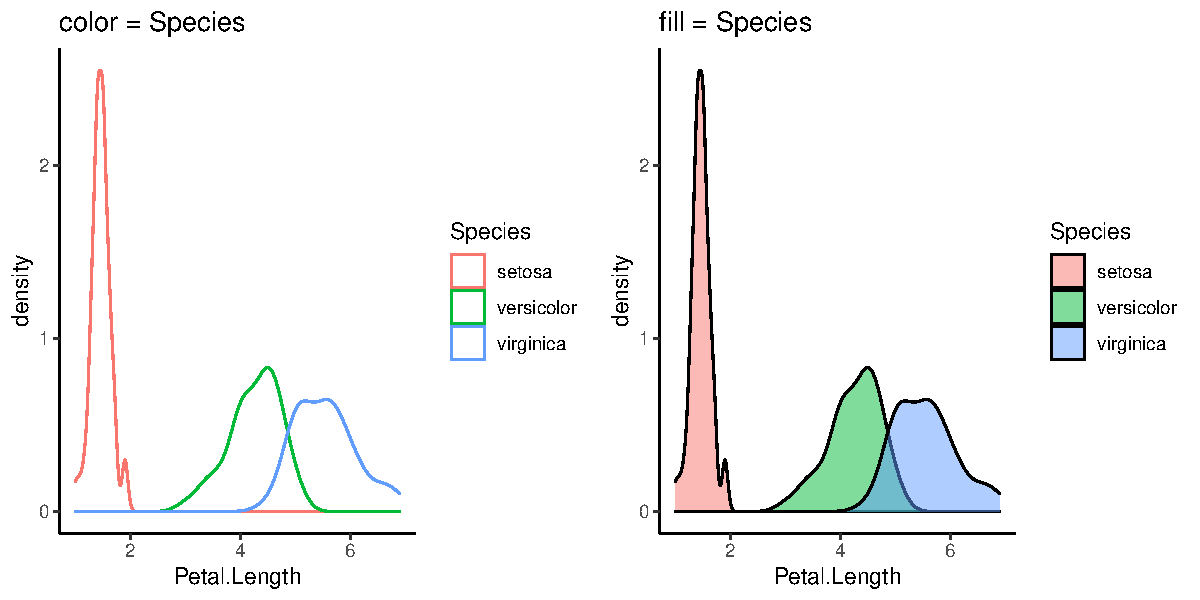
\includegraphics[width=0.99\linewidth]{PlotsLec2/denplt_ex1}
\caption{\small{Density plots of Petal.Length for three iris species using \textcolor{red}{\texttt{color = Species}} (\textit{left}) and \textcolor{red}{\texttt{fill = Species}} (\textit{right}).}}
\end{figure}
\end{frame}

\begin{frame}[fragile]\frametitle{RCode: \textcolor{red}{\texttt{color}} vs \textcolor{red}{\texttt{fill}} in \textcolor{red}{\texttt{geom}}$\_$\textcolor{red}{\texttt{density}}}
\lstset{basicstyle=\Large\ttfamily}
\begin{lstlisting}
# Petal.Length densities
base_plt <- ggplot(iris, aes(x = Petal.Length))

# color = Species
base_plt + geom_density(aes(color = Species))

# fill = Species
base_plt + geom_density(aes(fill = Species))
\end{lstlisting}
\end{frame}


\begin{frame}\frametitle{\textcolor{red}{\texttt{color}} vs \textcolor{red}{\texttt{fill}} in scatter plot}
\begin{figure}
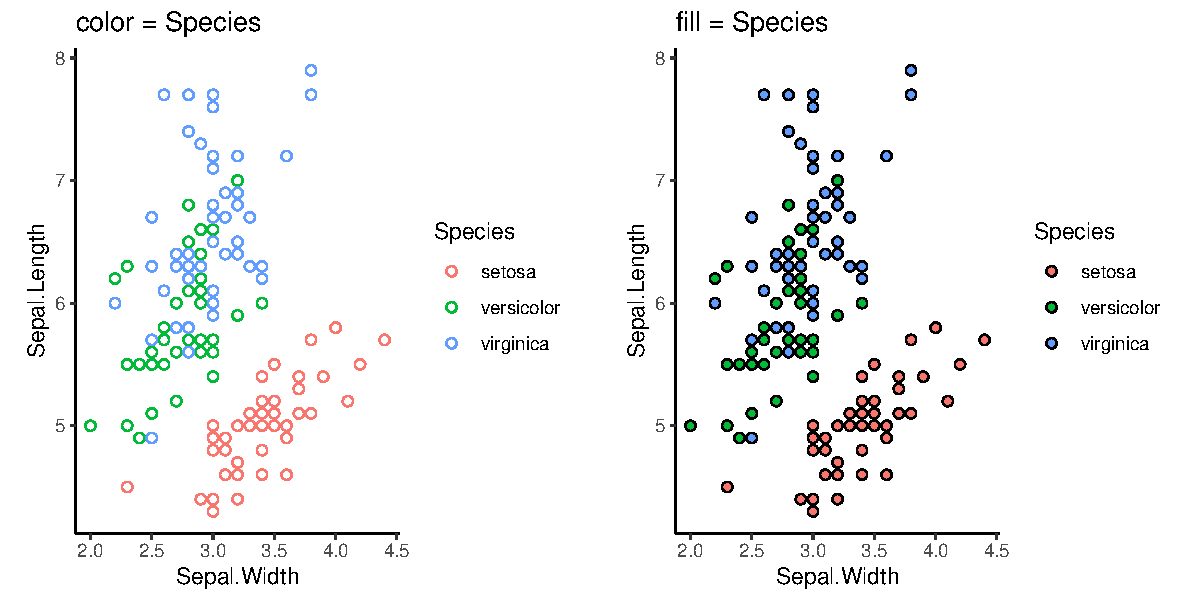
\includegraphics[width=0.99\linewidth]{PlotsLec2/scatplt_ex1}
\caption{\small{Scatter plots of Sepal.Length vs Sepal.Width using \textcolor{red}{\texttt{color = Species}} (\textit{left}) and \textcolor{red}{\texttt{fill = Species}} (\textit{right}); it is important to use a point \textcolor{red}{\texttt{shape}} that has both \textcolor{red}{\texttt{color}} and \textcolor{red}{\texttt{fill}} attributes.}}
\end{figure}
\end{frame}


\begin{frame}[fragile]\frametitle{RCode: \textcolor{red}{\texttt{color}} vs \textcolor{red}{\texttt{fill}} in \textcolor{red}{\texttt{geom}}$\_$\textcolor{red}{\texttt{point}}}
%\lstset{basicstyle=\Large\ttfamily}
\begin{lstlisting}
# Sepal.Length vs Petal.Length
base_plt <- ggplot(iris, aes(x = Petal.Length, y = Sepal.Length))

# color = Species
base_plt + geom_point(aes(color = Species), shape = 21)

# fill = Species
base_plt + geom_point(aes(fill = Species), shape = 21)
\end{lstlisting}
Note \textcolor{red}{\texttt{shape = 21}} outside the \textcolor{red}{\texttt{aes()}} function.
\end{frame}


\setbeamercovered{transparent}
\begin{frame}\frametitle{Aesthetics vs Attributes}
\begin{itemize}
\item It is common to confuse between \textcolor{red}{aesthetics mapping} and \textcolor{red}{visible attributes}.

\vspace{0.2in}

\item<2-> The confusion is often due to the fact that all \textcolor{red}{visual aesthetics} can be used as fixed \textcolor{red}{visible attributes}.

\vspace{0.2in}

\item<3-> \textcolor{red}{Fixed attributes} specify how \textcolor{red}{all plotting components should look}, e.g., colors of all points, size of all points, or transparency of all points. This is different than aesthetic mapping.

\vspace{0.2in}

\item<4-> To specify a fixed attribute, call it \textcolor{red}{outside} the \textcolor{red}{\texttt{aes()}} function.
\end{itemize} 
\end{frame}

\begin{frame}\frametitle{Common attributes: \textcolor{red}{\texttt{alpha}}, \textcolor{red}{\texttt{shape}} and \textcolor{red}{\texttt{size}}}

\begin{itemize}
\item In a scatter plot, the attributes \textcolor{red}{\texttt{alpha}}, \textcolor{red}{\texttt{shape}} and \textcolor{red}{\texttt{size}} can be controlled to produce better visualisation when there is overplotting (i.e., points lie on top of each other).

\vspace{0.1in}

\item \textcolor{red}{\texttt{alpha}} controls the transparency --- \textcolor{red}{\texttt{alpha = 0}} means completely transparent, while \textcolor{red}{\texttt{alpha = 1}} means completely opaque. A suitable value between 0 and 1 should be chosen.

\vspace{0.1in}

\item \textcolor{red}{\texttt{shape}} controls the point shape, e.g., \textcolor{red}{\texttt{shape = 1}} plots open circle, while \textcolor{red}{\texttt{shape = 21}} plots closed circle. 

\vspace{0.1in}

\item \textcolor{red}{\texttt{size}} controls the size of geom objects.
\end{itemize}

\end{frame}

\begin{frame}\frametitle{Example: \textcolor{red}{\texttt{alpha}} controls transparency}
\begin{figure}
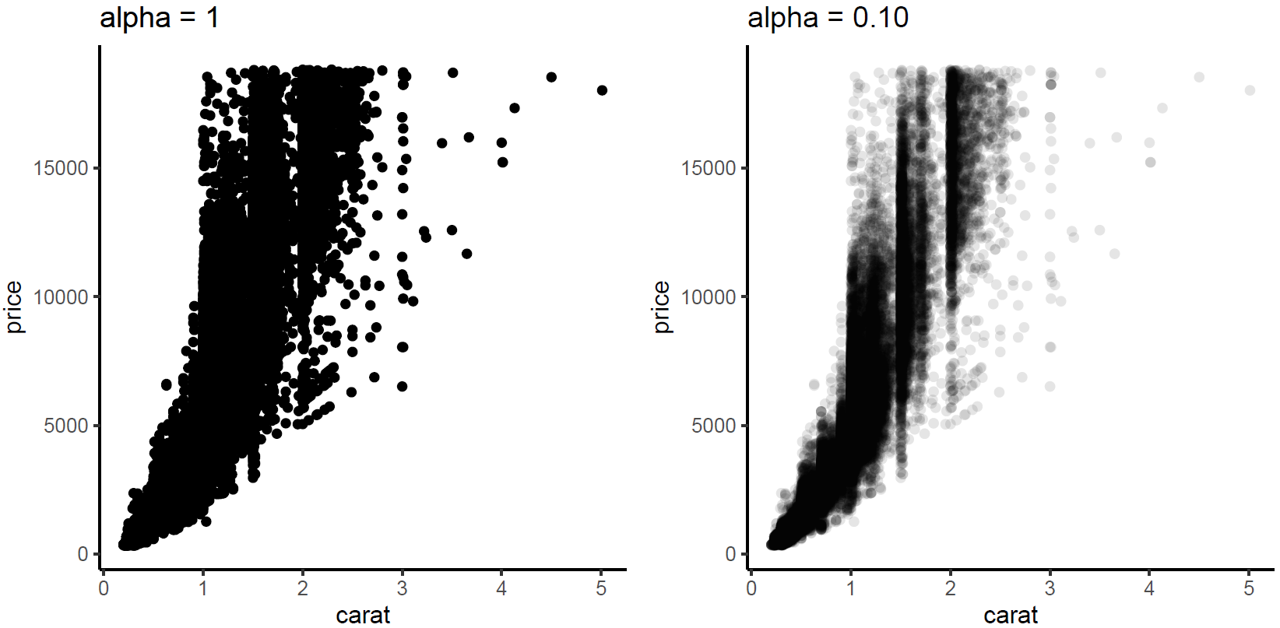
\includegraphics[width=0.99\linewidth]{PlotsLec2/diam_alpha2}
\caption{\small{Diamonds price plotted against carat (weight of the diamond between 0.2 and 5.01) using the \textcolor{red}{\texttt{diamonds}} dataset  from the \textcolor{red}{\texttt{ggplot2}} package.}}
\end{figure}
\end{frame}

\begin{frame}[fragile]\frametitle{RCode: \textcolor{red}{\texttt{alpha}} controls transparency}
\lstset{basicstyle=\Large\ttfamily}
\begin{lstlisting}
# price vs carat
base_plt <- ggplot(diamonds, aes(x = carat, y = price))

# alpha = 1
base_plt + geom_point()

# alpha = 0.10
base_plt + 
geom_point(alpha = 0.10)
\end{lstlisting}
\end{frame}

\begin{frame}\frametitle{Attributes: \textcolor{red}{\texttt{alpha}}, \textcolor{red}{\texttt{size}}, \textcolor{red}{\texttt{shape}}, and \textcolor{red}{\texttt{color}}}
\begin{figure}
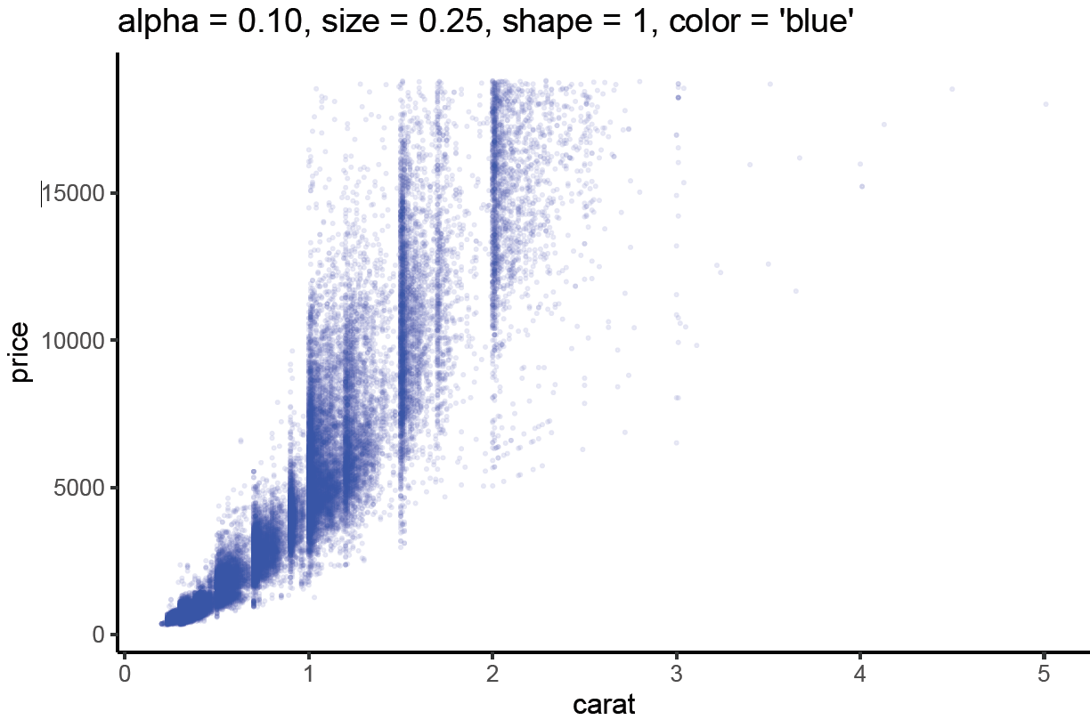
\includegraphics[width=0.99\linewidth]{PlotsLec2/diamonds2}
\caption{\small{Diamonds price plotted against carat using the \textcolor{red}{\texttt{diamonds}} dataset  from the \textcolor{red}{\texttt{ggplot2}} package.}}
\end{figure}
\end{frame}

\begin{frame}[fragile]\frametitle{RCode: \textcolor{red}{\texttt{alpha}}, \textcolor{red}{\texttt{size}}, \textcolor{red}{\texttt{shape}}, and \textcolor{red}{\texttt{color}}}
%\lstset{basicstyle=\Large\ttfamily}
\begin{lstlisting}
# price vs carat
base_plt <- ggplot(diamonds, aes(x = carat, y = price))

# alpha = 0.1, size = 0.25, shape = 1, color = 'blue'
base_plt +
 geom_point(alpha = 0.10, size = 0.25,
            shape = 1, color = "blue")
\end{lstlisting}
\end{frame}

\section{Key element-3: Geometry}
\begin{frame}\frametitle{Combining different \textcolor{red}{\texttt{geoms}}}
\Large
We can add one \textcolor{red}{\texttt{geom}} layer on top of another \textcolor{red}{\texttt{geom}} either using the same aesthetic mappings or different aesthetics.
\end{frame}

\begin{frame}\frametitle{Combining \textcolor{red}{\texttt{geom}}$\_$\textcolor{red}{\texttt{point}} and \textcolor{red}{\texttt{geom}}$\_$\textcolor{red}{\texttt{smooth}}}
\begin{figure}
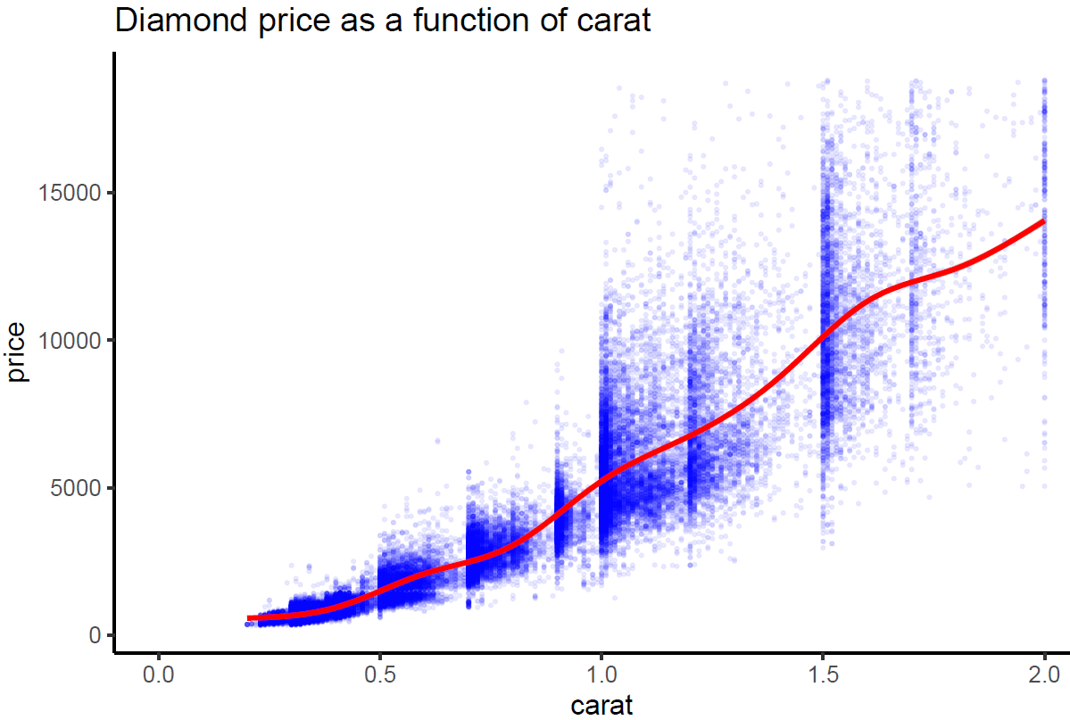
\includegraphics[width=0.99\linewidth]{PlotsLec2/GeomPointSmooth2}
\caption{\small{GAM used to predict diamond price as a function of carat.}}
\end{figure}
\end{frame}

\begin{frame}[fragile]\frametitle{RCode: \textcolor{red}{\texttt{geom}}$\_$\textcolor{red}{\texttt{point}} and \textcolor{red}{\texttt{geom}}$\_$\textcolor{red}{\texttt{smooth}}}

\begin{lstlisting}
# price vs carat
ggplot(diamonds, aes(x = carat, y = price)) +
# geom_point
geom_point(alpha = 0.10, size=0.25, shape=1, color = "blue") +
# geom_smooth
geom_smooth(color = "red") +
xlim(c(0, 2.0)) +
theme_classic() 
\end{lstlisting}
Note: Different visible attribute specifications in \textcolor{red}{\texttt{geom}}$\_$\textcolor{red}{\texttt{point()}} and \textcolor{red}{\texttt{geom}}$\_$\textcolor{red}{\texttt{smooth()}}.
\end{frame}

\begin{frame}\frametitle{Aesthetics in \textcolor{red}{\texttt{geom}}$\_$\textcolor{red}{\texttt{point}} and \textcolor{red}{\texttt{geom}}$\_$\textcolor{red}{\texttt{smooth}}}
\begin{figure}
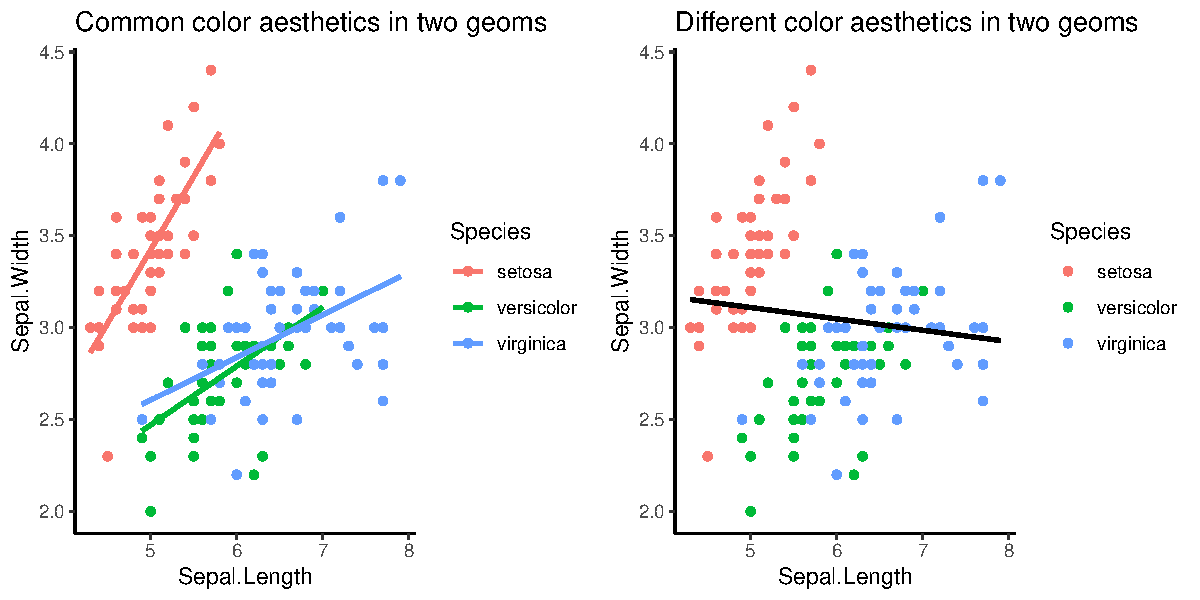
\includegraphics[width=0.99\linewidth]{PlotsLec2/scatter_aes_examples}
\caption{\small{\textit{Left}: Both geoms inherits same aesthetic mappings; \textit{Right}: Only \textcolor{red}{\texttt{geom}}$\_$\textcolor{red}{\texttt{point}} maps Species to color aesthetics.}}
\end{figure}
\end{frame}

\begin{frame}[fragile]\frametitle{Aesthetics in \textcolor{red}{\texttt{geom}}$\_$\textcolor{red}{\texttt{point}} and \textcolor{red}{\texttt{geom}}$\_$\textcolor{red}{\texttt{smooth}}}
\lstset{basicstyle=\small\ttfamily}
\begin{lstlisting}
############################################
# Same aes mapping in both geoms           #
############################################
ggplot(iris, aes(Sepal.Length, Sepal.Width, 
                 color = Species)) +
geom_point() +
geom_smooth(method = "lm", se = FALSE) +
theme_classic()
############################################
# color=Species only in geom_point()       #
############################################
ggplot(iris,aes(Sepal.Length,Sepal.Width)) +
geom_point(aes(color = Species)) +
geom_smooth(method = "lm", se = FALSE, color="black") +
theme_classic()
\end{lstlisting}
\end{frame}

\begin{frame}\frametitle{Combining \textcolor{red}{\texttt{geom}}$\_$\textcolor{red}{\texttt{boxplot}} and \textcolor{red}{\texttt{geom}}$\_$\textcolor{red}{\texttt{jitter}}}
Can you guess the aesthetic mappings? Also, can you spot a small problem with this plot?
\begin{figure}
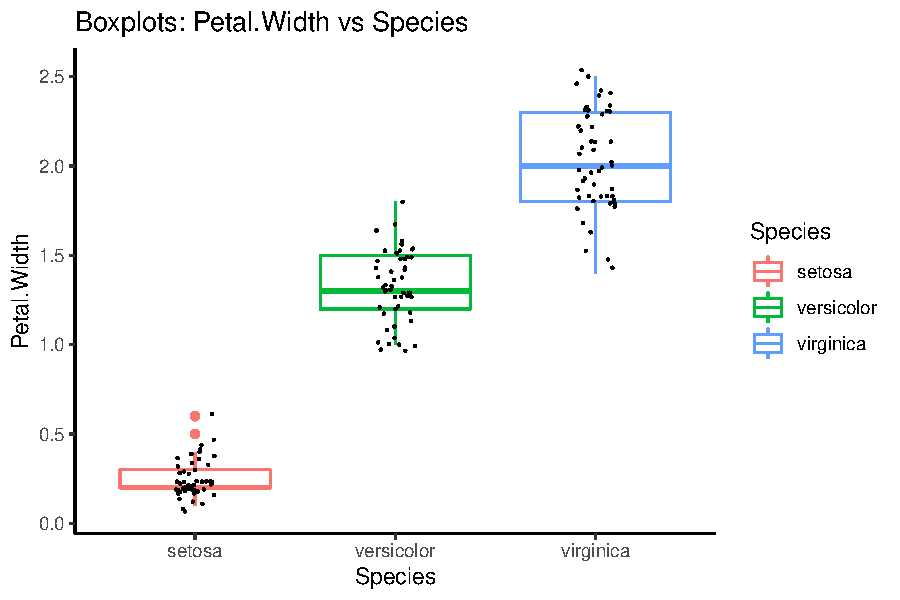
\includegraphics[width=0.99\linewidth]{PlotsLec2/GeomBoxJitter}
\end{figure}
\end{frame}

\begin{frame}\frametitle{Resolving the outlier colour and shape issue}
Use \textcolor{blue}{\texttt{outlier.color}} and \textcolor{blue}{\texttt{outlier.size}} in \textcolor{red}{\texttt{geom}}$\_$\textcolor{red}{\texttt{boxplot}} to modify outlier color and size, respectively.
\begin{figure}
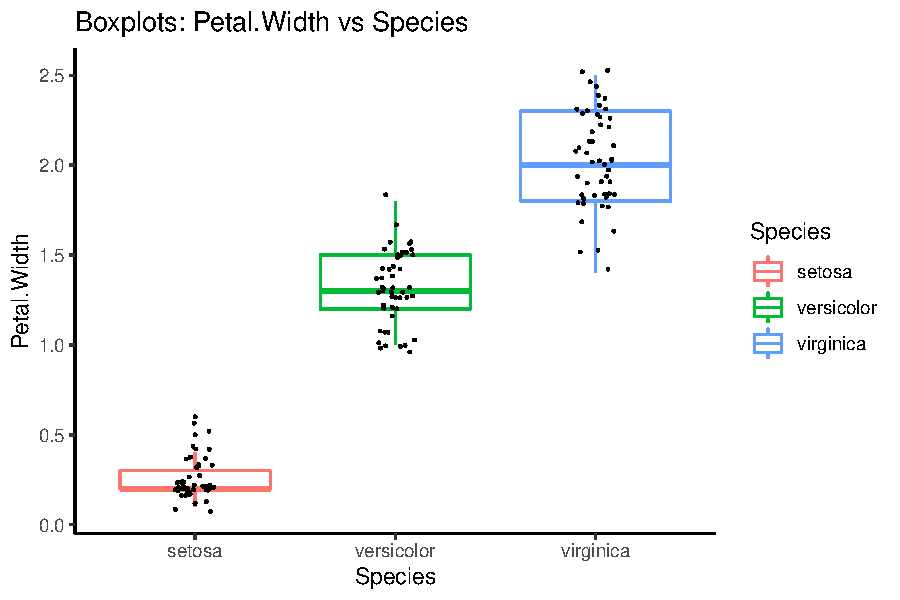
\includegraphics[width=0.99\linewidth]{PlotsLec2/GeomBoxJitter2}
\end{figure}
\end{frame}

\begin{frame}[fragile]\frametitle{RCode: \textcolor{red}{\texttt{geom}}$\_$\textcolor{red}{\texttt{boxplot}} and \textcolor{red}{\texttt{geom}}$\_$\textcolor{red}{\texttt{jiter}}}
%\lstset{basicstyle=\small\ttfamily}
\begin{lstlisting}
# Petal.Width boxplots for three species
ggplot(iris,aes(Species,Petal.Width)) +
# Map Species to color in geom_boxplot
geom_boxplot(aes(color = Species), 
             outlier.color = "black",
             outlier.size = 0.20) +
# Specify size and range of points
geom_jitter(size=0.20, width = 0.10) +
theme_classic()
\end{lstlisting}
\end{frame}

\begin{frame}\frametitle{A  few points on jittering}
\begin{itemize}
\item Jittered plot is an useful alternative to a scatter plot when there is overplotting.
\vspace{0.2in}

\item Because \textcolor{red}{\texttt{geom}}$\_$\textcolor{red}{\texttt{jitter()}} adds random noise to points, it may not be reproducible.

\vspace{0.2in}

\item To reproduce the same pattern, we should use \textcolor{red}{\texttt{set.seed()}} before calling \textcolor{red}{\texttt{geom}}$\_$\textcolor{red}{\texttt{jitter()}}.

\vspace{0.2in}

\item The other solution is to use \textcolor{red}{\texttt{position = }} \textcolor{red}{\texttt{position}}$\_$\textcolor{red}{\texttt{jitter(seed = 123)}} inside the \textcolor{red}{\texttt{geom}}$\_$\textcolor{red}{\texttt{point()}} function.
\end{itemize}
\end{frame}

\begin{frame}\frametitle{Example: combined geoms with faceting}
\begin{figure}
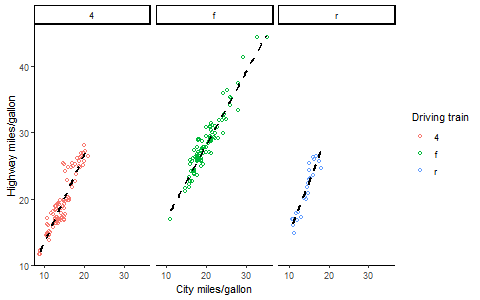
\includegraphics[width=0.99\linewidth]{PlotsLec2/hwy_cty_drv}
\caption{\small{\textcolor{red}{\texttt{hwy}} vs \textcolor{red}{\texttt{cty}} for three \textcolor{red}{\texttt{drv}}s.}}
\end{figure}
\end{frame}

\begin{frame}[fragile]\frametitle{RCode: combined geoms with faceting}
\begin{lstlisting}
ggplot(mpg, aes(x = cty, y=hwy)) +
# Reproduce jittering
geom_point(aes(color=factor(drv)), 
position = position_jitter(seed = 123),
shape = 1) +
# fit a linear regression
geom_smooth(method = "lm", se = FALSE, color="black", linetype = "dashed") +
# Faceting based on drv factor
facet_wrap(~ factor(drv)) +
theme_classic() +
labs(color = "Driving train",
     x = "City miles/gallon",
     y = "Highway miles/gallon")
\end{lstlisting}
\end{frame}

\section{Summary}
\begin{frame}\frametitle{Summary}
\begin{itemize}
\item Ggplot2 is built using the \textit{grammar of graphics}, and that makes it possible to build complex visualisations using the basic visualisation components.

\item Ggplot figures are built by adding visualisation layer on top of each other, and we can inspect a figure at any stage of this process and make decision about the next enhancement.

\item Three key components are data, aesthetic, and geometry.

\item There is a subtle difference between aesthetic mapping and visible attributes. 

\item Many geoms can be combined to produce complex visualisations.

\item Faceting is a great way to show the relationship between multiple variables.
\end{itemize}
\end{frame}


\end{document} 